% -*- root: ../AlgebraConmutativa.tex -*-
\chapter{Anillos I: nociones básicas}

Durante este curso vamos a trabajar mucho con anillos. Recordemos conceptos básicos vistos en Estructuras Algebraicas \cite{apuntesEA}.


\begin{defn}[Grupo]
Un grupo es un conjunto, G, con una operación binaria $'\cdot'$, que compone dos elementos $a \cdot b \in G$ para formar otro elemento notado como $a \cdot b$ o $ab$. Se escribe: $(G,\cdot)$. Para ser considerado grupo debe satisfacer:
\begin{enumerate}
	\item Cerrado: $\forall a,b \in G$, entonces $a \cdot b \in G$
	\item Asociatividad: $\forall a,b,c \in G$, entonces $(a\cdot b) \cdot c = a \cdot (b \cdot c)$
	\item Elemento neutro: $\exists e \in G$ tal que $\forall a \in G$ se cumple que $e\cdot a=a\cdot e = a$. A este elemento neutro se le denomina como elemento identidad o $1_G$.
	\item Elemento inverso: $\forall a \in G$ existe un elemento $b \in G$ tal que $a \cdot b = b \cdot a = e$. Sea $a \in G$, a su elemento inverso se le denomina $a^{-1}$.
\end{enumerate}
\end{defn}

\begin{defn}[Subgrupo]
Sea un grupo  $(G,\cdot)$, un subconjunto H de G es un subgrupo de G cuando H es un grupo con $\cdot$ restringida a los elementos de H. Por tanto, debe cumplir:
\begin{enumerate}
	\item H contiene al elemento identidad: $e \in H$.
	\item H es cerrado: $\forall a,b \in H$, entonces $a \cdot b \in H$.
	\item H contiene los elementos inversos: $\forall a \in H$ entonces $a^{-1} \in H$.
\end{enumerate}
\end{defn}

\begin{prop} \label{prop:def_subgrupo2}
Las tres condiciones anteriores son equivalentes a probar que $\forall a,b \in H$, entonces $a \cdot b^{-1}  \in H$.

\begin{proof}
Queremos ver que $\forall a,b \in H \implies a \cdot b^{-1}  \in H$ es equivalente a las tres condiciones anteriores.
\begin{itemize}
\item $\forall a,b \in H \text{ entonces } a \cdot b^{-1}  \in H \Rightarrow \text{ Las 3 condiciones anteriores }$
\begin{enumerate}
 \item H contiene al elemento identidad. Cogiendo $a \in H$ y $a \in H$, entonces $a \cdot a^{-1} \in H$. Y $a \cdot a^{-1} = e$ por definición.
 \item H contiene los elementos inversos: Sea $a \in H$ y $e \in H$ (que ya hemos visto que está), entonces $e \cdot a^{-1} \in H$. Y $e \cdot a^{-1}=a^{-1}$ por definición.
 \item H es cerrado: Sean $a,b \in H$ queremos ver que $a\cdot b \in H$. Como $b \in H$, entonces $b^{-1}\in H$ (por la propiedad anterior). Ahora cogemos $a,b^{-1} \in H$ y entonces $a\cdot (b^{-1})^{-1} \in H$.
\end{enumerate}
\item $ \text{ Las 3 condiciones anteriores } \Rightarrow \forall a,b \in H \text{ entonces } a \cdot b^{-1}  \in H $. Obvio
\end{itemize}
\end{proof}
\end{prop}


\begin{defn}[Subgrupo\IS normal]
	Un subgrupo normal N de un grupo G es un subgrupo invariante por conjugación; es decir, para cada elemento $n \in N$ y cada $g \in G$, el elemento $gng^{-1} \in N$ (Análogamente $Ng = gN$). N es un subgrupo normal de G se escribe $N \triangleleft G$
\end{defn}

\begin{defn}[Grupo\IS conmutativo]\index{Grupo!abeliano}
Un grupo $(G,\cdot)$ es conmutativo o abeliano si es un grupo y además la operación $\cdot$ es conmutativa. Es decir, $\forall a,b \in G, a\cdot b = b \cdot a$.
\end{defn}

\obs Si un subgrupo es conmutativo entonces también es un subgrupo normal.

\begin{defn}[Anillo] \label{def:Anillo}
Sea $R$ un conjunto no vacío, y sean $'+'$ y $'\cdot'$ dos operaciones binarias en $R$. Se dice que el conjunto $(R, +, \cdot )$ es un anillo si se cumplen las siguientes propiedades:

\begin{enumerate}
	\item $R$ es un grupo conmutativo con la primera operación $'+'$. Es decir, $(R,+)$ es un grupo conmutativo. Si utilizamos como primera operación la suma ($'+'$), al elemento neutro lo denotaremos por \zero.
	\item $R$ es cerrado con respecto a la segunda operación $'\cdot'$. Es decir $\forall a,b \in R$, entonces $a \cdot b \in R$
	\item $R$ es asociativo con respecto a la segunda operación $'\cdot'$. Es decir, $\forall a,b,c \in R$, entonces $(a\cdot b) \cdot c = a \cdot (b \cdot c)$
	\item La segunda operación $'\cdot'$ es distributiva con respecto a la primera $'+'$. Es decir, $a \cdot (b+c) = a\cdot b + a \cdot c$
	\[
	\left\{ \begin{array}{c}
	a \cdot (b+c) = a\cdot b + a \cdot c \\
	(b+c) \cdot a = b\cdot a + c\cdot a \\
	\end{array}
	\right.
	\]
\end{enumerate}
\end{defn}


\begin{defn}[Anillo\IS unitario]
	Se dice que un anillo $(R, +, \cdot)$ es unitario si tiene un elemento neutro respecto de la segunda operación $'\cdot'$. A ese elemento neutro lo denotaremos por \one):
	\[ x\cdot \one = \one \cdot x = x \]
\end{defn}

\begin{defn}[Anillo\IS conmutativo]
Se dice que un anillo $(R, +, \cdot)$ es conmutativo si la segunda operación $'\cdot'$ tiene la propiedad conmutativa:
\[ a\cdot b = b\cdot a \]
\end{defn}


\nota Durante el curso trabajaremos con anillos conmutativos con unidad (anillos conmutativos unitarios), aunque no se mencione de manera explícita.

\begin{example}
\begin{itemize}
	\item Anillo no conmutativo: matrices cuadradas.
	\item Anillo sin unidad: los pares en $\ent$.
\end{itemize}
\end{example}


\begin{example}
Anillos que utilizaremos:
\begin{itemize}
	\item $\ent$, $\ent_n$ $n \geq 1$ (casi siempre que pida un ejemplo, estará basado en ellos).
	\item $\rac$, $\real$, $\cplex$, $\field_{p^n}$.
	\item R anillo de polinomios: $R[x] = \set{ \sum_{i=0}^n a_i x^i \tq a_i \in R, n \in \nat}$. Dos expresiones en $R[x]$ son iguales $\iff$ los coeficientes son iguales uno a uno\ie $a_i = b_i \ \forall i$.
	\item R anillo de polinomios en n variables. Denotaremos como $R[x_1,\dots,x_n]$ a un anillo de polinomios con coeficientes en $R$ en $n$ variables:
	\[ R[x_1,\dots,x_n] = \set{ \sum_{i_1,\dots,i_n} a_{i_1,\dots,i_n} x^{i_1}\dots x^{i_n} \tq a_{i_1,\dots,i_n} \in R } \]
	\item $\ent_6$ es un anillo finito, mientras que $\ent_6[x]$ es infinito.
\end{itemize}
\end{example}


\nota Consideraremos que los $\nat$ contienen al 0.

\notacion Para abreviar en muchas ocasiones llamaremos $R$ a $(R,+,\cdot)$.

\begin{defn}[Unidades]\index{Elemento! invertible}
Sea $(R,+,\cdot)$. un anillo, se dice que $a\in R$ es invertible (también llamado unidad) ($a\in \U(R)$) si $\exists b\in R $ \st $a \cdot b = \one$. Es decir, tiene elemento inverso con respecto a la segunda operación $'\cdot'$.
\end{defn}

\begin{defn}[Unidades\IS de R: $\U(R)$]
Al conjunto de todas las unidades (o elementos invertibles) de un anillo R se le denomina $\U(R)$.
\end{defn}

\begin{defn}[Cuerpo]
Sea $(R,+,\cdot)$ un anillo, diremos que es un cuerpo si $R\setminus \set{0} = R^*$ es un grupo conmutativo con la segunda operación $'\cdot'$ \ie si todo elemento no nulo de $R$ es una unidad ($\U(R) = R^*$).
%, donde $R^* = R \setminus \set{0}$.
\end{defn}

\notacion Sea A un conjunto: $A\setminus \set{0} = A^*$

\begin{example} Ejemplos de cuerpos:
	\begin{itemize}
		\item $\rac, \real, \cplex, \field_{p^n}$ ($\ent$ no es un cuerpo) % si, los ejemplos se repiten
		\item $\rac[\sqrt2] = \set{ a + b\sqrt2 \tq a,b \in \rac }$
	\end{itemize}
\end{example}

\begin{prop}
	Si $\zero=\one$, entonces todos los elementos del anillo son 0.
\end{prop}

\begin{defn}[Divisor de cero]
Sea $(R,+,\cdot)$ un anillo. Se dice que $a \in R$, $a\neq\zero$, es un {\bf divisor de cero}, si $\exists b \in R$, $b \neq \zero$, \st $a\cdot b = \zero$.
\end{defn}

\begin{defn}[Nilpotente]
Se dice que $a\in R$ es nilpotente si $\exists n \in \nat$, $n\geq 1$, \st $a^n = \zero$.
\end{defn}

\begin{example}
	\begin{itemize}
		\item En $\ent_6$, $\cls{2} * \cls{3} = \zero$, y como tenemos que $\cls{2} \neq \zero, \cls{3}\neq \zero$, $\cls{2}\neq\cls{3}$, sabemos que $\cls{2}$ y $\cls{3}$ son divisores de cero.
		\item En $\ent_4$, $\cls{2}^2 = \zero \implies \cls{2}$ es nilpotente.
	\end{itemize}
\end{example}


\begin{lemma}
	Todo elemento nilpotente es divisor de cero.
\end{lemma}

\begin{proof}
	Sea A grupo y sea $a \in A$, $a\neq\zero$, elemento nilpotente y sea
		\[n = \min\set{n \tq a^n = \zero, n \in \nat}\]
	Luego $a^n = a * a^{n-1} = \zero$. Y tenemos que $\zero \neq b = a^{n-1} \in A$ es el elemento \st $a*b=\zero$ ya que como $a\neq \zero$, $a^n = \zero \implies n\geq 2 \implies a^{n-1} \neq \zero$.
\end{proof}

\begin{lemma}
	No todo divisor de cero es nilpotente.
\end{lemma}

\begin{proof} % los contraejemplos siempre son sencillos
	En $\ent_6$, $\cls{2}$ es divisor de $\zero$ pero no es nilpotente ya que:
	\begin{gather*}
		\cls{2}^0 = \cls{1}, \ \cls{2}^1 = \cls{2}, \ \cls{2}^2 = \cls{4}, \ \cls{2}^3 = \cls{2}, \ \cls{2}^4 = \cls{4}, \ \dots
	\end{gather*}
\end{proof}

\begin{defn}[Dominio\IS de integridad]
Diremos que R es un dominio si no tiene divisores de cero.
\end{defn}

\begin{example}
	$\ent$
\end{example}

\begin{defn}[Anillo\IS reducido]\label{def:AnilloReducido}
Diremos que R es un anillo reducido si no tiene elementos nilpotentes no nulos.
\end{defn}

\begin{example}
	\begin{itemize}
		\item Anillos reducidos que son dominios: $\ent, \ent_2$
		\item Anillo reducido que no es dominio: $\ent_6$
		\item Anillos no reducidos: $\ent_4$, $\ent_8$, $\ent_9$, \dots
	\end{itemize}
\end{example}

%\obs Las variedades algebraicas usan anillos reducidos: si el anillo es dominio, la variedad es reducible; si el anillo no es dominio, se dice que la variedad es no reducible.
% Y os preguntaréis, ¿Qué es una variedad algebraica? Pues hasta el tema 3...

\obs Si $a \in R$ divisor de cero, entonces $a$ \underline{\bf NO} es invertible. El recíproco también es cierto. (Las unidades y los divisores de 0 se llevan muy mal)

\obs Un anillo con unidad tiene al menos una unidad (el $\cls{1}$), y dos si $\cls{1} \neq \cls{-1}$. % nada que demostrar, la verdad

\begin{defn}[Subanillo]
Sea $(R,+,\cdot)$ un anillo y sea $S \subseteq R$, $S \neq \emptyset$. Diremos que $S$ es subanillo de $R$ si $S$ es un anillo con las operaciones definidas en $R$. Basta ver que:
\begin{enumerate}
	\item \one $\in S$
	\item $\forall a,b \in S$, entonces $a-b \in S$
	\item $\forall a,b \in S$, entonces $a\cdot b \in S$
\end{enumerate}
\end{defn}



\begin{example} Ejemplos de subanillos.
	\begin{enumerate}
		\item $R \subset R[x]$
		\item $\ent \subset \rac \subset \real \subset \cplex$
		\item Ningún $\ent_n$ es subanillo de $\ent$, porque $\ent_n \not \subseteq \ent$. Esto es así porque ni siquiera $\ent_n$ es un subconjunto de $\ent$ ya que los elementos de $\ent$ no son los mismo que los de $\ent_n$, en el primer caso son números normales y corrientes, y en el segundo son $\{\cls{i},  \forall 0 < i < n$, y representan el resto de dividir $i$ entre $n$.
		% porque en $\ent$, 4 y 6 son distintos, pero en $\ent_n$ pueden ser iguales
	\end{enumerate}
\end{example}


\begin{defn}[Ideal] \label{def:Ideal} % no, no se refiere a un modelito
Sea $(R,+,\cdot)$ un anillo y sea $I \subseteq R$. Se dice que $I$ es un ideal si:

	\begin{enumerate}
		\item $I \neq \emptyset$
		\item $(I, +)$ es un subgrupo de R.
		\item \concept{Propiedad de absorción}: $\forall i \in I, \forall r \in R \implies r\cdot i \in I$.
	\end{enumerate}
\end{defn}

\obs Como $R$ es abeliano con  $'+'$ por definición, entonces si $(I,+)$ es un subgrupo, entonces es un subgrupo normal.
% Revisado. Guille.

\obs Cualquier ideal contiene al \zero. Ya que es el elemento neutro del subgrupo $(I,+)$.

\begin{defn}[Ideal\IS propio]
	Decimos que un ideal $I \subseteq R$ es propio si $I \neq R$.
\end{defn}

\begin{example} Ejemplos de ideales:
	\begin{itemize}
		\item Fijado $k \in \ent$, el conjunto $\set{n\cdot k \tq n \in \nat }$ es un ideal de $\ent$.
		\item En $R$, hay siempre dos ideales, R (que es un ideal no propio) y $\set{0}$.
		\item En $\ent_{10}$, $[\cls{0},\cls{2},\cls{4},\cls{6},\cls{8} ]$ forman un ideal.
	\end{itemize}
\end{example}

\begin{example} Sea $\rac[x,y]$, sea $J=\{p(x,y): p(1,1)=0\}$ es un ideal. Lo comprobamos:
\begin{enumerate}
	\item $J \neq \emptyset$ porque $0 \in J$
	\item $(J,+)$ es un subgrupo.

	Hay que comprobar que J contiene al 0 (elemento neutro) que es cerrado con $'+'$ y que contiene los elementos inversos, pero como hemos visto esto es equivalente a probar que $\forall p(x,y), q(x,y) \in J$, entonces $p(x,y)-q(x,y) \in J$ (ya que con la suma, el inverso de $q(x,y)$ es $-q(x,y)$).

	Como $p(1,1)=0=q(1,1)$, evidentemente $p(1,1)-q(1,1)=0$ y por tanto $p(x,y)-q(x,y) \in J$.
	\item Si escogemos $r(x,y) \in \rac[x,y]$ y si $p(x,y) \in J$, tenemos que ver que $r(x,y)\cdot p(x,y) \in J$. Obvio ya que $p(1,1)=0 \implies r(1,1)\cdot p(1,1) = 0$
\end{enumerate}
\end{example}

Las siguientes dos observaciones son muy \textbf{IMPORTANTES} y se utilizan mucho, son referentes a ideales. Sea $I \subseteq R$ un ideal de un anillo R:
\begin{itemize}
	\item Si $\one \in I \implies I=R$. Por la propiedad de absorción.
	\item Si $u\in I$ siendo u una unidad $\implies I=R$. Ya que si u es una unidad, entonces por la propiedad de absorción, cogiendo $r=u^{-1} \in R$ obtenemos \one (el elemento neutro respecto a $'\cdot'$).
\end{itemize}
\begin{prop}
	$R$ es un cuerpo $\iff$ los únicos ideales de $R$ son $\zerogen$ y $R$.
\end{prop}
\begin{proof}

	$\Leftarrow$) Sea $a \in R$, $a \neq 0$, queremos probar que $\exists a' \in R$ tal que $aa' = 1$ \footnote{Es decir, la definición de cuerpo, que todo elemento de $R$ es una unidad.}.

	Consideramos $I=\set{ra \tq r \in R}$ y vamos a ver que es un ideal. Está claro que $I \neq \zerogen$ ya que $a \in I$ \footnote{Cogiendo $r = \one$.}. Por tanto, como por hipótesis tenemos que $R$ solo tiene dos ideales, queda que $I=R$, y como $\one \in R$, entonces $\one \in I$, y por la propiedad de absorción, existe un $r$ tal que $ra=1$.

	$\Rightarrow$) Supongamos $\exists I$ ideal propio de $R$ distinto de $\zerogen$, y sea $a \in I$ tal que $a \neq \zero$. Por la propiedad de absorción, $\one \in I$ ya que $a*a^{-1} = \one$; luego, de nuevo, por la propiedad de absorción, tenemos que $I = R$. $\Rightarrow\Leftarrow$

	Luego el único ideal propio de $R$ es $\zerogen$, y $R$ siempre es un ideal de $R$.
\end{proof}

Se pueden deducir las siguientes 2 definiciones alternativas de ideal:

\begin{prop}\label{prop:def_ideal2}
	Sea $(R,+,\cdot)$ un anillo y sea $I \subseteq R$. Se dice que $I$ es un ideal si

	\begin{enumerate}
		\item $I \neq \emptyset$
		\item $\forall a,b \in I$, entonces $a-b \in I$.
		\item Propiedad de absorción
	\end{enumerate}
\end{prop}
\begin{prop}\label{prop:def_ideal3}
	Sea $(R,+,\cdot)$ un anillo y sea $I \subseteq R$. Se dice que $I$ es un ideal si

	\begin{enumerate}
		\item $I \neq \emptyset$
		\item $\forall a,b \in I$, entonces $a+b \in I$.
		\item Propiedad de absorción
	\end{enumerate}
\end{prop}


Más aún podemos ver que:
\begin{prop}
	La definición original de ideal es equivalente a
	la proposición \ref{prop:def_ideal2} es equivalente a la proposición \ref{prop:def_ideal3}.
\end{prop}
\begin{proof}
	\begin{itemize}
		\item De la definición original a la proposición \ref{prop:def_ideal2} solo cambia el segundo punto. Pero como ya hemos visto (proposición \ref{prop:def_subgrupo2}), son equivalentes.
		\item De la la proposición \ref{prop:def_ideal2} a la proposición \ref{prop:def_ideal3}, usamos que $-1 \in R$ siempre porque es el inverso de $\one$ que siempre pertenece a $R$. Por tanto, usanda la propiedad de absorción $(-1)b=-b \in I$ y por tanto $a-(-b)=a+b \in I$.
	\end{itemize}
\end{proof}


\begin{lemma}
 Sea R un anillo, el conjunto de los elementos nilpotentes de R es un ideal que recibe el nombre de \concept{nilradical} de R. Que denotaremos por $\nil(R)$.
\end{lemma}
\begin{proof}
	\begin{itemize}
		\item $\nil(R) \neq \emptyset$ porque $\zero \in \nil(R)$
		\item Sean $a,b \in \nil(R)$ tenemos que ver que $a+b \in \nil(R)$:

		Como $a \in \nil(R)$ entonces $\exists n$ tal que $a^n=0$.\\
		Como $b \in \nil(R)$ entonces $\exists m$ tal que $b^m=0$.

		Por tanto:
		$$(a+b)^{n+m} = \sum_{j=0}^{n+m} \binom{n+m}{j} a^j \cdot b^{n+m-j} = 0$$

		Ya que si $j<n$ se anula b, y si $j \geq n$ se anula a.
		\item Sea $a \in \nil(R)$ y sea $r\in R$, queremos ver si $ra \in \nil(R)$.

		Como $a\in \nil(R) \implies \exists n \geq 1 \st a^n=0$, por tanto $(ra)^n = 0$ (recordemos que trabajamos con anillos conmutativos).
	\end{itemize}
\end{proof}

\begin{prop}
	R es reducido $\Leftrightarrow$ $\nil(R)=\set{0}$
\end{prop}


\begin{prop}
	Sea $T \subseteq R$, $T \neq \emptyset$, existe un ideal en $R$ tal que es el más pequeño que contiene a $T$.
\end{prop}
\begin{proof}
	Basta considerar la intersección de todos los ideales que contienen a $T$; que no puede ser vacía porque al menos, el ideal $R$ contiene a $T$.
\end{proof}

\begin{defn}[Ideal\IS generado por T]
Definimos el ideal generado por $T$ como el ideal más pequeño de $R$ que contiene a $T$ y se denota por $\gen{T}$.

Explícitamente, sea $R$ un anillo y $T \subset R$ no vacío, entonces:
$$ \gen{T} = \{r_1t_1+...+r_st_s: r_i \in R, t_i \in T, s \geq 1 \} $$
\end{defn}

La notación no es arbitraria, recordamos que $\gen{E}$ es el subespacio vectorial generado por $E$. Más adelante descubriremos que, filosóficamente, son la misma cosa.

\begin{example} Sea $\rac[x,y]$, y sea $T=\{x,y\}$, entonces el ideal generado por T es:
	$$\gen{T} = \gen{x,y} = \{p(x,y)\cdot x+q(x,y)\cdot y : p(x,y),q(x,y) \in \rac[x,y]\}$$
\end{example}

\section{Operaciones con Ideales}

\begin{prop}
	Sea $\{J_i\}_{i\in I}$ una familia de ideales en $R$. Entonces $\bigcap_{i \in I}J_i$ es un ideal.
\end{prop}


\begin{prop}
	Sean $I,J \subset R$ ideales, entonces $I \cup J$ en general no es un ideal.
\end{prop}

\begin{example} En $\ent$
	Sean $\gen{2}$ (los pares) y $\gen{3}$ (múltiplos del 3). Ambos son ideales, sin embargo $J=\gen{2} \cup \gen{3}$ no es un ideal.

	Esto es así porque $3\in \gen{3}$, $2 \in \gen{2}$ y sin embargo $3-2=1$, que no pertenece a $\gen{2} \cup \gen{3}$, por tanto, $(J,+)$ no es subgrupo de $\ent$, y por tanto $J$ no es ideal de $\ent$
\end{example}

\begin{defn}[Ideal\IS más pequeño que contiene a dos ideales] \label{def:IdealSuma}
Sean $I$ y $J$ ideales, entonces llamamos $I+J$ al ideal más pequeño que contiene a I y a J, que explícitamente es:
$$ I+J = \{a+b: a\in I, b\in J\} $$

%\textcolor{red}{No pillo esto, si cogemos el ejemplo no veo la diferencia entre $\gen{2} \cup \gen{3}$ y $\gen{2} + \gen{3}$, ambos contienen los mismos elementos no?}

%\noteby{Guille}{No es exactamente lo mismo. $\gen{2} ∪ \gen{3}$ contiene los elementos que son múltiplos de 2 y/o de 3. Sin embargo, $\gen{2} + \gen{3}$ va a contener precisamente a elementos como el $1$ que nos destrozaban antes el ejemplo, ya que $1 = 3 + (-2)$ con $3 ∈ \gen{3},\, -2 ∈ \gen{2}$. También contendrá otros como 5, 8, que son sumas de múltiplos de 2 y 3. De hecho, como $1 ∈ \gen{2} + \gen{3}$ tenemos que $\gen{2} + \gen{3} = ℤ$, creo.}

\end{defn}

\begin{defn}[Producto\IS de ideales] \label{def:IdealProducto}
	Sean $I$ y $J$ dos ideales, entonces $J\cdot I = \gen{a\cdot b: a \in I, b \in J}$

	En general, sea $I=\gen{f_1,\dotsc ,f_s}$ y $J=\gen{g_1,\dotsc,g_t}$ entonces:
	$$I\cdot J=\gen{ f_i, g_j: i \in \{1,...,s\}, j \in \{1,...,t\}}$$
\end{defn}

\begin{example} Sea $\gen{x,y} \subset \real[x,y]$
	$$\gen{x,y}^2 = \gen{x^2,xy,y^2}$$
\end{example}

\obs Dados $I,J \subset R$ no es cierto que todo elemento $h \in I\cdot J$ sea igual al producto de un elemento de $I$ por otro de $J$.

\begin{example}
	Sea $I=J=\gen{x,y}$, entonces $I\cdot J = \gen{x^2,xy,y^2}$.

	Cogemos el elemento $x^2 + y^2$ perteneciente a $I\cdot J$. Podemos ver que $x^2 + y^2$ no se puede escribir como $p(x,y) \cdot q(x,y)$ con $p(x,y),q(x,y) \in \gen{x,y}$. (Y con $p(x,y)$ o $q(x,y)$ distintos de 1)

	\obs En los complejos sí se podría ya que $(x+iy)(x-iy)=x^2 + y^2$
\end{example}

\obs Sean $I$ y $J$ dos ideales, se cumple que $I\cdot J \subseteq I$ y que $I \cdot J \subseteq J$, y por tanto $I \cdot J \subseteq I \cap J$. En general esta última inclusión es estricta.

\begin{example}
	\begin{itemize}
\item Inclusión estricta: en $\ent$, cogemos $I=\gen{2}$, $J=\gen{4}$. Tenemos que $I\cdot J=\gen{8}$ pero $I\cap J=\gen{4}$.
\item Inclusión no estricta: en $\ent$, cogemos $I=\gen{2}$, $J=\gen{3}$. Tenemos que $I\cdot J=\gen{6}$ pero $I\cap J=\gen{6}$.
	\end{itemize}
\end{example}

\begin{defn}[Radical\IS de un ideal] \label{def:RadicalIdeal}
Sea $I \subset R$ un ideal. Definimos el radical de I como:
$$\mop{Rad}(I)=\sqrt{I}=\{a \in R: \exists n \in \nat \textbf{ con } a^n \in I \}$$
\end{defn}

\begin{example}
\begin{itemize}
	\item En $\ent$: $\sqrt{\gen{2}}=\gen{2}$, $\sqrt{\gen{4}}=\gen{2}$, $\sqrt{\gen{8}}=\gen{2}$, $\sqrt{\gen{6}}=\gen{6}$
	\item En $\rac[x,y]$: $\sqrt{\gen{x^2,xy}}=\gen{x}$
\end{itemize}
\end{example}

\begin{defn}[Ideal radical]
	Sea $I\subset R$ un ideal. Se dice que es radical si $I=Rad(I)$.
\end{defn}

\textcolor{blue}{\obs $\rac[x,y]$ es dominio de factorización única. (ya definiremos y hablaremos de esto más adelante)}

Veamos algunas observaciones referentes al radical de un ideal. Sea $I \subset R$ un ideal. Entonces:
\begin{itemize}
	\item $I \subset \mop{Rad}(I)$
	\item $\mop{Rad}(I)$ es un ideal
	\item $\{\text{Elementos nilpotentes }\}=\nil(R)=\{a\in R: \exists n \text{ con }a^n=0 \}=\mop{Rad}((0))$
\end{itemize}

\begin{defn}[Ideal\IS primo] \label{def:IdealPrimo}
	Diremos que un ideal $I\subset R$ es primo si $I\neq R$ y si cada vez que $a\cdot b \in I$ se tiene que $a\in I$ o $b\in I$.
\end{defn}

\begin{example} En $\ent$
	\begin{itemize}
		\item $\gen{p}$ con p primo es un ideal primo.
		\item (0) es un ideal primo.
	\end{itemize}
\end{example}

\begin{example} En $\ent_6$
	\begin{itemize}
		\item (\zero) no es ideal primo. Ya que $\cls{2} \cdot \cls{3}=\cls{0}=\zero$
		\item $\gen{\cls{2}}=\{\cls{0},\cls{2},\cls{4} \}$ es un ideal primo.
		\item $\gen{\cls{3}}=\{\cls{0},\cls{3} \}$ es un ideal primo.
	\end{itemize}
\end{example}

\begin{prop}
	Sea $K$ un cuerpo, y sea $K[x]$, entonces $\gen{x}$ es primo.
\end{prop}
\begin{proof}
	Tenemos que $K[x]$ es un dominio de factorización única  Consideramos el ideal generado por $x$, es decir: $\gen{x}$.

	%(\textcolor{red}{No se esto para que lo usa} \noteby{Guille}{Creo que para decir que $p(x)q(x) = x·r(x)$ y por lo tanto $x$ divide a $p(x)$ o a $q(x)$. Si no fuese DFU $xr(x)$ podría tener otra factorización alternativa y no sabríamos en cuál de las dos se cumple que $x$ divide a alguno de los factores.}).

	Supongamos que $p(x)\cdot q(x) \in \gen{x}$. Entonces, por ser un ideal, por la propiedad de absorción $\exists r(x) \in K[x]$ tal que $p(x) q(x)=r(x) x$. Por tanto, necesariamente $x|p(x)$, y en ese caso $p(x) \in \gen{x}$, o $x|q(x)$, y en ese caso $q(x) \in \gen{x}$.
\end{proof}

Generalizamos la proposición anterior:
\begin{prop}
	Sea K un cuerpo, y sea $K[x_1,...,x_n]$, entonces $\gen{x_i}$ es primo.
\end{prop}

\begin{prop}
	Sea K un cuerpo, y sea $K[x_1,...,x_n]$, se cumple que si $\gen{p(x_1,...,x_n)}$ es primo,  entonces $p(x_1,...,x_n)$ es irreducible.
\end{prop}

\begin{example}
	En $\real[x]$: $\gen{x^2+1}$ es primo y $p(x)=x^2+1$ es irreducible.
\end{example}

\begin{prop}\label{prop:def_idealGeneradoxy}
	Sea $K$ un cuerpo (Esto es cierto también si $K$ es un anillo que no sea cuerpo, confirmado por Ana), y sea el ideal $\gen{x,y}$ en $K[x,y]$, entonces:
	$$\gen{x,y}=\{p(x,y)\in K[x,y]:p(0,0)=0 \}$$
\end{prop}

\begin{proof}
	\begin{itemize}
		\item $\subset)$ Hemos visto que $\gen{x,y}=\{s(x,y) x+r(x,y) y: s(x,y),r(x,y) \in K[x,y] \}$. Es obvio que $s(x,y) x+r(x,y) y$ se anula en el $(0,0)$.
		\item $\supset)$ Sea $p(x,y) \in K[x,y]$ tal que $p(0,0)=0$. Tenemos que $p(x,y)=a_0+a_1x+a_2y+a_3x^2+...+a_nx^ny^m$. Entonces $p(0,0)=a_0=0$. Por tanto, si $a_0=0$, entonces $p(x,y)$ se puede expresar como $r(x,y)y+s(x,y)x$.
	\end{itemize}
\end{proof}

\obs De esta forma, podemos probar (siendo K un cuerpo) que $\gen{x,y} \in K[x,y]$ es un ideal primo de forma más sencilla. Supongamos que $p(x,y)q(x,y) \in \gen{x,y}$, necesariamente $p(x,y) \in \gen{x,y}$ o $q(x,y) \in \gen{x,y}$. Ya que como $p(x,y)q(x,y) \in \gen{x,y}$ entonces $p(0,0)q(0,0)=0$, pero como K es un cuerpo (y un dominio de integridad), no tiene divisores de 0, por tanto debe cumplirse que $p(0,0)=0$ o que $q(0,0)=0$.

\obs Y si no es cuerpo no tiene porque ser primo ya que puede ser que los dos coeficientes independientes de p y q, llamémosles $a_p$ y $a_q$ sean distintos de 0 y $p(0,0)q(0,0)=a_pa_q=0$, por ejemplo en $\ent_6$ con $a_p=\cls{2}$ y $a_q=\cls{3}$.

Se deja como ejercicio para el lector experimentado probar que en $K[x_1,...,x_n]$, (K cuerpo) el ideal $\gen{x_1-a_1,...,x_n-a_n}$ con $a_1,...,a_n \in K$, es primo.

\begin{defn}[Ideal\IS maximal] \label{def:IdealMaximal}
	Sea $I \subsetneq R$ un ideal (propio), diremos que I es un ideal maximal si cada vez que encontremos un ideal $J ⊆ R$ con $I \subset J$, se tiene que o bien $I=J$ o bien $J=R$.

	En otras palabras $I$ es un ideal maximal si $I \subsetneq R$  (propio) y es maximal respecto a la inclusión de ideales.
\end{defn}

\begin{example}
	\begin{itemize}
		\item En $\ent$ son maximales los $\gen{p}$ con p primo.
		\item En $\ent_8$ hay los siguientes ideales:
		\begin{itemize}
			\item $\gen{\cls{2}}=\{\cls{0},\cls{2},\cls{4},\cls{6} \}$ que es el único maximal
			\item $\set{\cls{0}}$ que no es maximal por estar contenido en $\gen{\cls{2}}$.
			\item $\ent_8$ que no es maximal porque no es propio.
			\item $\gen{\cls{4}}=\{\cls{0},\cls{4} \}$ que no es maximal por estar contenido en $\gen{\cls{2}}$.
		\end{itemize}
	\end{itemize}
\end{example}

\begin{defn}[Ideal\IS principal]\label{def:ideal_principal}
	Un ideal es principal si está generado por un único elemento.
\end{defn}

\begin{example}
	Sea $R$ un anillo, el ideal principal generado por un elemento $a \in R$ es el conjunto:
	$$ \gen{a}=(a)=\{ra: r \in R \} $$
\end{example}

\begin{prop}
	Sea $K$ un cuerpo, y sea $K[x]$, todos los ideales de $K[x]$ son principales. $K[x]$ es un dominio de ideales principales, es decir, todos los ideales están generados por un polinomio.
\end{prop}

\begin{prop}
Sea $K$ un cuerpo, y sea $p(x)\neq 0 \in K[x]$. $\gen{p(x)}$ es maximal $\Leftrightarrow$ $p(x)$ es irreducible.
\end{prop}

\begin{example}
Sea $\rac[x,y]$, cogemos el ideal $I=\gen{x-1,y-2}$, vamos a ver que es maximal.

\begin{proof}
	Supongamos que $I \subsetneq J$ para algún ideal $J \subset \rac[x,y]$. Osea que existe un $p(x,y) \in J$ pero $p(x,y) \notin I$

	Hacemos el desarrollo de Taylor de $p(x,y)$:

	$$ p(x,y)=p(1,2) + \underbrace{\left.\od{p(x,y)}{x}\right|_{(1,2)} (x-1)+ \left.\od{p(x,y)}{y}\right|_{(1,2)} (y-2)+\frac{1}{2}\left.\od[2]{p(x,y)}{x}\right|_{(1,2)} (x-1)^2+ \dotsb }_{\in \gen{x-1,y-2}}$$

	Osea que $p(x,y)=p(1,2)+r(x,y)$ con $r(x,y) \in \gen{x-1,y-2}$.

	Por tanto nos queda $\underbrace{p(1,2)}_{\in \rac^*}=\underbrace{\underbrace{p(x,y)}_{\in J}-\underbrace{r(x,y)}_{\in I \subset J}}_{\in J}$

	$p(1,2)$ es una constante no nula porque sino $p(x,y) \in I$. (Recordar que $\rac^*=\rac\setminus\{0\}$).

	Entonces, $p(1,2) \in \rac^*$ y $p(1,2) \in J =\rac[x,y]$

	Y nos queda que $I=\{ q(x,y) \in \rac[x,y]: q(1,2)=0 \}$
\end{proof}
\end{example}

Generalizamos una proposición anterior:
\begin{prop}
	Sea $K$ un cuerpo (Esto es cierto también si K es un anillo que no sea cuerpo, confirmado por Ana), y sea el ideal $<x_1-a_1,...,x_n-a_n>$ contenido en $K[x_1,...,x_n]$, entonces:

	$$\gen{x_1-a_1,...,x_n-a_n}=\set{p(x_1,...,x_n)\in K[x_1,...,x_n]:p(a_1,...,a_n)=0 }$$
\end{prop}

\begin{theorem} \label{thm:IdealContenidoMaximal}
	Sea $R$ un anillo y sea $I \subsetneq R$ un ideal, entonces $I$ está contenido en un maximal de $R$.
\end{theorem}
\begin{proof}
Vamos a usar el Lema de Zorn:
\begin{lemma}[Lema\IS de Zorn] \label{lem:Zorn}
Sea $\Sigma$ un conjunto no vacío parcialmente ordenado. Si toda cadena creciente de elementos de $\Sigma$ tiene una cota superior, entonces $\Sigma$ tiene un elemento maximal.
\end{lemma}

Definimos $\Sigma = \{J \subsetneq R \text{ ideal }: I\subseteq J \}$. Tenemos que:
\begin{itemize}
	\item $\Sigma \neq 0$ ya que $I \in \Sigma$.
	\item $\Sigma$ está parcialmente ordenado con la inclusión de ideales.
	\item Si $\{ J_n\}$ es una cadena creciente de ideales ($J_n \subset J_m$ $\forall m\geq n$), vamos a comprobar que la cadena está acotada en $\Sigma$.
\end{itemize}
Sea $H = \bigcup J_n$. Queremos ver que $H \in \Sigma$, es decir, que es un ideal y que $I \subset H$. Si así lo fuese está claro que $H$ sería una cota superior (contiene a todos los $J \in \Sigma$) y podríamos aplicar el Lema de Zorn para decir que $\Sigma$ tiene un elemento maximal.

\begin{itemize}
	\item Sabemos que $H \neq \emptyset$ ya que $0 \in J_n \forall n$, ya que el ideal más pequeño de todos es el $\set{0}$, además el elemento \zero pertenece a todos los ideales. Por tanto $\zero \in H$.
	\item Sean $a,b \in H=\bigcup J_n$.  Entonces $\exists m,k \in \nat$ tal que $a \in J_m$ y $b \in J_k$. Sin pérdida de generalidad supongamos que $m \geq k$. Entonces $a,b \in J_m$, y por tanto $a+b \in J_m \subset H$.
	\item Como ejercicio para el lector experimentado se deja comprobar la propiedad de absorción. Si $r\in R$ y $a \in H$, entonces $ra \in H$.
\end{itemize}
Cumplidas esas tres condiciones, hemos demostrado que H es un ideal.

Además, por construcción $I \subset H$, ya que $I \subset J_n \; \forall n$.

Veamos ahora que $H \neq R$. Supongamos para llegar a una contradicción que $H=R$. Entonces $\one \in H$, por tanto, $\exists m$ tal que $\one \in H$. Pero es imposible ya que $J_m \in \Sigma$ (si $1 \in J_m$ entonces $J_m$ sería igual a R, y en $\Sigma$ eso no puede ocurrir).

Por tanto llegamos a una contradicción. Entonces $H \in \Sigma$ y aplicando Zorn, $\Sigma$ tiene un elemento maximal.
\end{proof}

\begin{prop}
	Todo anillo tiene al menos un elemento maximal
\end{prop}
\begin{proof}
	Tomar $I=\set{0}$ en el teorema anterior.
\end{proof}

\obs Un caso extremo es cuando $R$ es un cuerpo, en ese caso $\set{0}$ es el único ideal propio, y por tanto es el único maximal.

Veremos más adelante que todo ideal maximal es primo, y por tanto este teorema dice que en todo anillo $R$ hay ideales primos.

\begin{prop}
	Si en un anillo $R$ todos los ideales son primos, entonces $R$ es un cuerpo.
\end{prop}

\begin{example}
\begin{itemize}
\item $\ent_9:$ $\gen{\cls{3}} =\{\cls{0},\cls{3},\cls{6} \}$ es el único ideal maximal (por tanto es primo). ($\set{0}$ no es primo)
\item En $\ent$ hay infinitos maximales $\gen{p}$ con $p$ primo.
\item En $K[x]$, K cuerpo, hay infinitos maximales $\gen{p(x)}$ donde $p(x)$ es irreducible.
\end{itemize}
\end{example}

\obs Sea R un anillo en el que sólo hay un ideal maximal $I$. Entonces, si $\alpha \notin I$, usando el teorema anterior tenemos que $\gen{\alpha}=R$, ya que si $\gen{\alpha}\subsetneq R$ tendríamos que está contenido en algún ideal maximal y sólo hay uno y $\alpha \notin I$. Como conclusión, de $\gen{\alpha}=R$ deducimos que $\alpha$ es unidad.

\begin{defn}[Anillo\IS local]
	Diremos que $R$ es un anillo local si solo tiene un ideal maximal.
\end{defn}

\begin{example}
	\begin{itemize}
	\item Cualquier cuerpo.
	\item $\ent_9$
	\item $\ent_{p^n}$ con $p$ primo: $\gen{\cls{p}}$
	\end{itemize}
\end{example}

\begin{example}
 Sea:
 $$ R=\set{ \frac{a}{b} : \frac{a}{b}\equiv \frac{a'}{b'} \text{ con } b' \notin 3\ent } $$

$R$ es un anillo. Queremos ver que es un anillo local, es decir, que tiene un único maximal.

Vamos a buscar ese maximal. Podemos ver qué elementos son unidades en R. Por ejemplo 3 no es unidad, ya que $\frac{1}{3} \notin R$, sin embargo 2 sí es unidad ya que $\frac{1}{2} \in R$ y $\frac{1}{2}\cdot 2 = \one$.

Definimos:
$$ m = \set{\frac{a}{b} \in R ¡: \frac{a}{b} \equiv \frac{a'}{b'}\text{ con }b'\notin 3\ent, a' \in 3\ent }$$

Se puede probar que $m$ es ideal, pero hay que ver que es el único ideal maximal.

Sin embargo, todo $r\in R$ con $r \notin m$ es una unidad, ya que si $r \notin m \implies r=\frac{a}{b}$ de modo tal que $a,b\notin 3\ent$, lo que implica que $r^{-1}\equiv \frac{b}{a} \in R$.Esto implica que todo elemento $r \notin m$ cumple que $\gen{r} =R$. Por tanto $m$ es maximal.
\end{example}

\begin{defn}[Anillo\IS semilocal]
 Si $R$ tiene un número finito de maximales se dice que R es semilocal
\end{defn}

Vamos a ver qué sucede si consideramos la intersección de todos los ideales primos de un anillo:
\begin{example}
	\begin{itemize}
		\item En $\ent$: $\displaystyle\set{0} \bigcap_{p\in \ent\text{ primo}}\gen{p}=\set{0}$
		\item En $\ent_4$: sólo tenemos $\gen{\cls{2}}$
		\item En $\ent_6$: $\gen{\cls{2}}\cap\gen{\cls{3}}=\set{0}$
		\item En $\ent_{12}$: $\gen{\cls{2}}\cap\gen{\cls{3}}=\set{6}$
	\end{itemize}
\end{example}

\begin{prop}
	Sea $R$ un anillo, entonces:
	$$ \nil(R)=\bigcap_{\substack{p\subset R\\\text{p ideal primo}}} p $$

\end{prop}
\begin{proof}

\proofpart{$\subset$}

	Sea $a \in \nil(R) \implies \exists n$ tal que $a^n=0$ y $0 \in p$, $\forall p \subset R$, p primo. Queremos ver que $a \in p$.

	Si $n=1$, obvio, ya que tendríamos $a=0\in p\; \forall p \subset R$ ideal primo.

	Si $n>1$, entonces $a^n = a\cdot a^{n-1}=0 \in p$ para cualquier $p$ ideal primo. Por ser $p$ primo, o $a$ o $a^{n-1}$ pertenecen a p. Si $a$ está en $p$, paramos porque es lo que queríamos demostrar. Si no, hacemos el mismo argumento con $a^{n-1}$ e iterando llegaremos a que $a \in p$, $\forall p \subset R$, $p$ ideal primo.

\proofpart{$\supset$}

	Para ver que $\bigcap_{p\subset R \text{ p ideal primo }}p \subset \nil(R)$ vamos a probar que si $b \in R$ no es nilpotente, entonces existe un primo $p\subset R$ tal que $b \notin p$.

	Sea $b \in R$, no nilpotente entonces:
	$$\Sigma = \{I \subseteq R \text{ ideal, tal qye }b^n \notin I, \forall n \in \nat\}$$, tenemos que:
	\begin{itemize}
	\item $\Sigma \neq \zero$ porque $(\zero) \in \Sigma$.
	\item $\Sigma$ está ordenado parcialmente con la inclusión de ideales.
	\item Si $\{I_n\}$ es una cadena creciente de ideales, en $\Sigma$, vamos a ver que está acotada en $\Sigma$, basta tomar $\bigcup I_n$, que pertenece a $\Sigma$.
	\end{itemize}

	Aplicando el Lema de Zorn, $\Sigma$ tiene un elemento maximal, llamémoslo $a \subsetneq R$ ideal, y además $b^n \notin q \forall n$.

	Vamos a probar que q es primo. Sean $\alpha, \beta \in R$, tal que $\alpha, \beta \notin q$. Entonces:
	-$q \subsetneq q + <\alpha>$ (Ideal más pequeño que contiene a $q$ t a $\alpha$)
	-$q \subsetneq q + <\beta>$ (Ideal más pequeño que contiene a $q$ t a $\beta$)

	Por tanto, $ q + <\alpha>$ y $q + <\beta>$ no pertenecen a $\Sigma$.

	Por tanto:
	-$\exists n\geq 1$ tal que $b^n \in q+<\alpha>$ (quiere decir que $b^n=c+r_1 \alpha$, $c\in q$)
	-$\exists m\geq 1$ tal que $b^m \in q+<\beta>$ (quiere decir que $b^m=d+r_2 \beta$, $d\in q$).

	Y nos quedaría que:
	$$b^{n+m}=\underbrace{cd}_{\in q}+\underbrace{cr_2\beta}_{\in q}+\underbrace{dr_1\alpha}_{\in q}+r_1r_2\alpha \beta$$

	Entonces:
	$$b^{n+m}\in q+<\alpha \beta> \notin \Sigma$$

\end{proof}

\begin{defn}[Ideal\IS primo minimal]
	Diremos que un ideal primo $p \subsetneq R$ es minimal si cada vez que otro ideal primo $q \subsetneq R$ esta contenido en p, entonces q=p.
\end{defn}

\begin{example}
	\begin{itemize}
		\item En $\ent$: el $\set{0}$ es un primo minimal y lo mismo sucede en cualquier dominio de integridad.
		\item En $\ent_6$: $\gen{\cls{2}}$ y $\gen{\cls{3}}$ son minimales y maximales.
		\item En $\ent_n$ todo ideal maximal es también primo minimal.
		\item En $\rac[x,y]/\gen{x,y}$, $\gen{x},\gen{y}$ son primos minimales. De hecho estos primos minimales corresponden con las componentes irreducibles de las variedades  algebraicas afines. Como eso y nada me dicen lo mismo, pensad que $\gen{x}$ e $\gen{y}$ son básicamente los ejes de coordenadas de una gráfica de dos dimensiones. De todas formas profundizaremos en esto más adelante.
	\end{itemize}
\end{example}

\obs Si hay primos minimales, entonces:
$$ \nil(R)=\bigcap_{\substack{p\subset R \\ \text{ p primo }}} p = \bigcap_{\substack{p\subset R \\ \text{ p primo minimal }}}p $$

\section{Homomorfismos de anillos}

\begin{defn}[Homomorfismo\IS de anillos] \label{def:Homomorfismo} Sean $R$ y $S$ anillos y sea $\appl{f}{R}{S}$ una función. Diremos que F es un homomorfismo de anillos si:
\begin{enumerate}
	\item $\forall a,b \in R$, $f(a+b)=f(a)+f(b)$.
	\item $\forall a,b \in R$, $f(ab)=f(a)f(b)$
	\item $f(1_R)=1_S$ (Esta última propiedad no siempre se pide)
\end{enumerate}
\end{defn}

\begin{example}
	\begin{itemize}
		\item $f:\ent \rightarrow R$. Solo puedo construir un único homomorfismo de $\ent$ en cualquier anillo $R$. Ya que el 1 genera a $\ent$ como grupo aditivo, así que también genera al anillo. En este caso sería el homomorfismo dado por $f(1)=\one$ y $f(n)=nf(1)$.
		\item $f: \rac[x] \rightarrow \cplex$. Podríamos definir varios homomorfismos de anillos:
		\begin{align*}
			f: \rac[x] & \longmapsto  \cplex \\
			 1 & \longmapsto  1\\
			 m & \longmapsto  m \quad \forall m \in \ent\\
			 \frac{1}{m} & \longmapsto  \frac{1}{m} \quad \text{para } m\neq 0 \text{ Ya que } 1=m\frac{1}{m}=f(m)f(\frac{1}{m})=1\\
			 \frac{n}{m} & \longmapsto  \frac{n}{m} \quad \text{para }n,m \in \ent \text{ , } m\neq 0\\
			 x & \longmapsto  \text{ lo que quiera }\\
		\end{align*}
		\begin{itemize}
			\item $f(1)=1$
			\item $f(m)=m$, $\forall m \in \ent$
			\item $f(\frac{1}{m})=\frac{1}{m}$, para $m\neq 0$. Ya que $1=m\frac{1}{m}=f(m)f(\frac{1}{m})=1$
			\item $f(\frac{n}{m})=\frac{n}{m}$, para $n,m \in \ent$, $m\neq 0$
			\item $f(x)=$lo que quiera.
		\end{itemize}
		 Tendríamos un homomorfismo diferente dependiendo de a donde llevemos la variable x.
		 \item $f: \rac[\sqrt[3]{2}]\rightarrow \cplex$. Tenemos que $\rac[\sqrt[3]{2}] = \{a+b\sqrt[3]{2}+c\sqrt[3]{2^2}:a,b,c \in \rac\}$. En este caso tendríamos tres homomorfismos diferentes. Dejamos $\rac$ fijo, si $r\in \rac$, y con $w=e^{\frac{2\pi i}{3}}$ (raíz cúbica de la unidad):
		 \begin{enumerate}
		 	\item $f(r)=r$ y $f(\sqrt[3]{2})=\sqrt[3]{2}$
		 	\item $f(r)=r$ y $f(\sqrt[3]{2})=\sqrt[3]{2}w$
			 \item $f(r)=r$ y $f(\sqrt[3]{2})=\sqrt[3]{2}w^2$
		 \end{enumerate}
		 \item $f: \rac \rightarrow \ent$, no puedo construir un homomorfismo de anillos de $\rac$ en $\ent$. Ya que no podría definir la imagen de $1/2$ por ejemplo.
		 \item $f: \rac[\sqrt{2}]\rightarrow \rac[\sqrt{3}]$, tampoco existe un homomorfismo de anillos, ya que no hay ningún elemento en $\rac[\sqrt{3}]$ tal que su cuadrado sea 2.
	\end{itemize}
\end{example}

Ahora vamos a nombrar algunas propiedades de los homomorfismos de anillos:

Tenemos que recordar que un homomorfismo de anillos es antes que nada un homomorfismo de grupos. Sea $\appl{f}{R}{S}$ un homomorfismo de anillos:
\begin{enumerate}
\item $f(0_R)=0_S$
\item $f(-a)=-f(a)$
\item Si $u \in R$ es una unidad, entonces $f(u)$ es unidad y además $f(u^{-1})=f(u)^{-1}$
\item El núcleo de $f$, o $\ker(f)=\{ r \in R: f(r)=0 \}$, es unidad en $R$.
\end{enumerate}

\begin{prop}\label{prop:hda_inyectiva}
	$f$ es inyectiva $\Leftrightarrow$ $\ker (f)=\{0_R \}$
\end{prop}

\begin{defn}
	$\appl{f}{R}{S}$ es un isomorfismo (de anillos) si $f$ es homomorfismo biyectivo.
\end{defn}

\begin{prop}
	Si $f$ es homomorfismo de anillos biyectivo entonces se puede comprobar que $f^{-1}$ también es un homomorfismo de anillos
\end{prop}

\begin{defn}[Ideal\IS generado por $f(I)$]
	Sea $\appl{f}{R}{S}$ un homomorfismo de anillos, el ideal generado por $f(I)$, que denotaremos mediante $f(I)^e$, diremos que es el ideal $f(I)$ extendido en $S$.
\end{defn}

\subsection{Homomorfismos e ideales}
Sea $\appl{f}{R}{S}$ un homomorfismo de anillos:
\begin{enumerate}
	\item Sea $I \subset R$ un ideal, en general $f(I)$ no es un ideal en $S$.
	\begin{example}
		Sea $i:\ent \rightarrow \rac$, sea $I=2\ent$, entonces $i(I)$ no es un ideal en $\rac$. Vimos que un homomorfismo de $\ent$ en $R$ esta generado por el \one. No se cumple la propiedad de absorción, ya que por ejemplo, sea $\frac{1}{2} \in \rac$ y $f(2)=2 \in i(I)$, entonces $\frac{1}{2}\cdot2=1 \notin i(I)$.

		Podemos decir que $i(I)^e=\rac$.
	\end{example}
	\item Sea $J \subset S$ un ideal. Entonces, conjunto $f^{-1}(J)$ es un ideal.

	El $0_R$ por tanto pertenece a $f^{-1}(J)$.
	\begin{example}
		Sea $j: \ent \rightarrow \ent[x]$

		Cogemos $J=\gen{x}$, entonces $j^{-1}(J)=(0)$, más que nada porque no queda otra: como ha de ser $j(1) = 1$, luego $j(ℤ) = ℤ ⊂ ℤ[x]$. Por lo tanto, no queda ``hueco'' para que haya elementos en $ℤ$ cuya imagen sea $\gen{x}$ salvo el $0$, que está en $\gen{x}$ y que cumple que $j(0) = 0$.
	\end{example}
	\obs $\forall J \subset S$ entonces $f^{-1}(J)\supset \ker(f)$.
	\begin{prop}
		Si $\appl{f}{R}{S}$ es sobreyectiva, entonces $f(I)$ es un ideal en $S$, $\forall I \subset R$ ideal.
	\end{prop}
	\item Sea $\appl{f}{R}{S}$. Sea $I \subset R$ un ideal, podemos coger $f(I)^e$. Entonces $I\subseteq f^{-1}(f(I)^e)$ (En general el contenido es estricto).

	Y sea $J \subset S$ ideal, entonces $f(f^{-1}(J))^e \subseteq J$ (en general el contenido es estricto)
\end{enumerate}

\section{Anillos cociente}
\begin{defn}[Relación\IS de equivalencia]
	Sea $K$ un conjunto dado no vacío y $\algb{R}$ una relación binaria definida sobre $K$, se dice que $R$ es una relación de equivalencia si cumple las siguientes propiedades:
	\begin{enumerate}
		\item Reflexividad: Todo elemento de $K$ está relacionado consigo mismo, es decir,
		\[ \forall x \in K: x \algb{R} x \]
		\item Simetría: Si un elemento de $K$ está relacionado con otro, entonces ese otro elemento también se relaciona con el primero, es decir,
		\[ \forall x,y \in K: x \algb{R} y \implies y \algb{R} x \]

		\item Transitividad:  Si un elemento de K está relacionado con otro, y ese otro a su vez se relaciona con un tercero, entonces el primero estará relacionado también con este último. Es decir,
		\[ \forall x,y,z \in K: x \algb{R} y \wedge y \algb{R} z \implies x \algb{R} z \]
	\end{enumerate}
\end{defn}

\begin{defn}[Clase\IS de equivalencia]
	Dado un elemento $a\in K$, al conjunto dado por todos los elementos relacionados con $a$, se le llama clase de equivalencia asociada al elemento $a$:
	$$ \cls{a}=[a] = \{b\in K \tq b\mathcal{R}a\} $$
\end{defn}

\begin{defn}[Conjunto\IS cociente]
	Sea $A$ un conjunto y $\rel$ una relación de equivalencia. Entonces las clases de equivalencia por $\rel$ forman una partición del conjunto $A$. Por tanto, el conjunto cociente es el conjunto de todas las clases de equivalencia.
\end{defn}


Sea $R$ un anillo, y sea $I\subset R$ un ideal.

En $R$ definimos la siguiente relación: $a,b \in R$, $a \sim b$ si $a-b \in I$. Es fácil comprobar que es una relación de equivalencia (cumple las propiedades reflexiva, transitiva y simétrica).

Al conjunto cociente lo denotamos por $\quot{R}{I}$. Recordemos que $I$ es un subgrupo normal del grupo aditivo $R$.

Vamos a definir la suma y el producto de elementos del conjunto cociente:

\begin{itemize}
	\item Suma: Si tomamos $\cls{a}, \cls{b} \in R/I$, puedo sumar $\cls{a}+\cls{b}$ haciendo la suma en $R$, es decir, $a+b$. y luego tomando la clase, es decir, $\cls{a+b}$. Por tanto:
	$$ \cls{a}+\cls{b} = \cls{a+b} \implies \text{ con la suma tengo un grupo }$$
	\item Producto: tenemos que $ \cls{a}\cdot\cls{b} = \cls{a\cdot b} $.

	Cogemos un representante de $\cls{a}=a+I$ y otro de $\cls{b}=b+I$ y multiplicamos:
	$$ (a+I)(b+I)=ab+\underbrace{aI+bI+I}_{\in I} $$

	Como vemos, solo con un subanillo no funciona, necesito la propiedad de absorción de los ideales.
\end{itemize}

Por tanto, esto prueba que:
$$(R/I,+,\cdot) \text{ es un anillo conmutativo con unidad }$$

\begin{prop}\label{prop:pi_homomorfismo}
	La aplicación $\appl{\pi}{R}{\quot{R}{I}}$ es un homomorfismo de anillos. La demostración sale de la definición de suma y producto en $\quot{R}{I}$.
\end{prop}

\obs $\pi$ es sobreyectiva y $\ker(\pi)=I$

Vamos a ver ahora la \textbf{relación entre los ideales de $R$ y los de $\quot{R}{I}$}: \label{relacionRconRI}
\begin{enumerate}
	\item Sea $J \subset \quot{R}{I}$ un ideal, entonces $\pi^{-1}(J)$ es un ideal de $R$, además $\pi^{-1}(J)\supset I$.
	\item Sea $L \subset R$ un ideal, entonces $\pi(L) \subset R/I$ es siempre un ideal de $\quot{R}{I}$, porque $\pi$ es sobreyectiva.
	\item Sea $\pi: R \rightarrow \quot{R}{I}$.

	Sea $L\subseteq R$ ideal, entonces $\pi^{-1}(\underbrace{\pi(L)}_{\text{ideal en R/I}})$ contiene a $L$ y a $I$. A $I$ lo contiene por la propiedad 1, y a L por definición de función (sea $f:R \rightarrow S$, siempre $\forall B \in R$, $f^{-1}(f(B))\supset B$).

	Entonces $\pi^{-1}(\pi(L)) \supset (L+I)$. Recordemos que $L+I$ es el ideal más pequeño que contiene a $L$ e $I$.
	\begin{example}
		Sea $f: \ent \rightarrow \ent_6$. Entonces:
		\begin{itemize}
			\item $f(\gen{5})=\gen{\cls{5}}=\ent_6$.

			Por lo que acabamos de ver: $f^{-1}(f(\gen{5})) \supset \gen{5}$ y en $\gen{6}$. Entonces $\gen{5} + \gen{6} = \ent$ (Ya que el $m.c.d(5,6)=1$)
			\item $f(\gen{4})=\gen{\cls{4}}=\{\cls{0},\cls{4},\cls{2} \}$.

			Por lo que acabamos de ver: $f^{-1}(f(\gen{4})) \supset \gen{4}$ y en $\gen{6}$. Entonces $\gen{5} + \gen{6} = \gen{2}$ (Ya que el $m.c.d (4,6)=2$)
		\end{itemize}
	\end{example}

	\begin{prop}
		De hecho $\pi^{-1}(\pi(L)) = L+I$
	\end{prop}

	\begin{proof}
		Basta probar que $\pi^{-1}(\pi(L)) \subseteq L+I$, ya que es obvio que $L+I ⊆ \inv{π}(π(L))$. Sea $a \in \pi^{-1}(\pi(L))$, entonces $\pi(a) \in \pi(L)$ y por lo tanto $\exists b\in L$ tal que $\pi(a)=\pi(b)$ o, en otras palabras, que $b$ y $a$ pertenecen a la misma clase de equivalencia.

		Así, podemos operar y ver que $\pi(a)-\pi(b)=\pi(a-b)=0$, luego $a-b \in \ker \pi = I  \implies a=b+\alpha$, con $b \in L$ y $\alpha \in I$.
	\end{proof}

	%% Clase 8/2

	% Nota: yo esto lo habría puesto en un párrafo a parte fuera del enumerate, pero sigo el formato Parra.
	% Parra: XD.., no sé como queda mejor la verdad..
	\item Sea:
	\begin{align*}
		\appl{π}{R&}{\quot{R}{I}} \\
		L &\longmapsto \pi(L) \\
	\end{align*}

	Entonces, si $I \subset L$, por la propiedad 3, nos queda que: $\pi^{-1}(\pi(L))=L+I=L$.

	\item Supongamos que $L, M ⊂ R$ son ideales con $I ⊆ M \subsetneq L$. En ese caso, lo que querremos ver será la siguiente propiedad: $π(M) \subsetneq π(L)$.

	\begin{proof}
	Como $M \subsetneq L$, entonces existe un $l ∈ L$ que no está en $M$. Vamos a tratar de hacer la demostración por reducción al absurdo, suponiendo que $π(L) = π(M)$. En este caso, tendríamos que $π(l) ∈ π(L) = π(M)$, y por lo tanto ha de existir un $m ∈ M$ tal que $π(l) = π(m)$.

	Que $π(l) = π(m)$ implica que ambos elementos están en la misma clase de equivalencia, por lo tanto $l = m + α$ para algún $α ∈ I$. Sin embargo, como $m ∈ M$ y $α ∈ I ⊆ M$, $l$ es la suma de dos elementos de $M$ y por lo tanto ha de ser $l ∈ M$, contradicción porque se suponía que $M \subsetneq L$.
	\end{proof}

	La conclusión de esto es que hay una correspondencia biyectiva entre los ideales de $R$ y los de $\quot{R}{I}$, que además respeta inclusiones. Además, los maximales de $\quot{R}{I}$ se corresponderán con ideales maximales en $R$ que contengan a $I$. Estas propiedades nos permitirán simplificar la búsqueda y entendimiento de ideales al poder pasar de un lado a otro.

	\begin{example}
	Vamos a estudiar los ideales de $ℤ$ y los de $\quot{ℤ}{6ℤ}$. En $ℤ$, los ideales que contienen a $\gen{6}$ son él mismo, el total ($\gen{1}$) y los de elementos que dividen a $6$, esto es, $\gen{2}$ y $\gen{3}$.

	La correspondencia entre estos ideales de $ℤ$ y los de $\quot{ℤ}{6ℤ}$ son sencillas: $\gen{6} \to (0)$, $\gen{1} \to Z_6$ y además $\gen{2} \to \set{\cls{2}, \cls{4}, \cls{0}}$ y $\gen{3} \to \set{\cls{3}, \cls{0}}$, siendo estos dos últimos, ideales maximales de $ℤ_6$.

	Así, podríamos ver qué es $π(\gen{4}) = π(\gen{4} + \gen{6}) = π(\gen{2})$, es decir, un maximal de los que habíamos visto antes.
	\end{example}
\end{enumerate}

Veremos ahora las herramientas que nos proporcionan estas propiedades y que nos permitirán trabajar con ideales primos, maximales y radicales.

\begin{prop}\label{prop:3_propiedades_anillos_cocientes}
Sea $I ⊂ R$. Entonces
\begin{enumerate}
\item $I$ es un ideal primo si y sólo si $\quot{R}{I}$ es un dominio de integridad (sin divisores de cero).
\item $I$ es maximal si y sólo si $\quot{R}{I}$ es un cuerpo.
\item $I$ es un ideal radical si y sólo si $\quot{R}{I}$ es reducido (sin nilpotentes).
\end{enumerate}
\end{prop}

\begin{proof}

\proofpart{$I$ primo $\iff$ $\quot{R}{I}$ es un D.I}

Por definición un \nlref{def:IdealPrimo} cumple que, cada vez que $ab ∈ I$, o bien $a ∈ I$ o bien $b ∈ I$. En nuestro caso, esto será equivalente a que si $\cls{ab} = \cls{0}$ en $\quot{R}{I}$, entonces $\cls{a} = 0$ o $\cls{b} = 0$, luego $\quot{R}{I}$ es un dominio de integridad.

\proofpart{$I$ maximal $\iff$ $\quot{R}{I}$ cuerpo}

Si $I$ es un \nlref{def:IdealMaximal}, entonces cada vez que $I$ está contenido en otro ideal $J$, o bien es $I = J$ o bien $J = R$. Traducido al cociente, tenemos que si $(\cls{0}) ⊂ \quot{J}{I}$, entonces o bien $(\cls{0}) = \quot{I}{I}$ o bien $(\cls{0}) = \quot{R}{I}$. Así, en $\quot{R}{I}$ sólo hay 2 ideales, $(\cls{0})$ y $\quot{R}{I}$, luego es un cuerpo.

\proofpart{$I$ radical $\iff$ $\quot{R}{I}$ reducido}

Si $I$ es radical, entonces si $f^n ∈ I$ para algún $n$, se tiene que $f ∈ I$. Por lo tanto, si $\cls{f}^n = \cls{0}$ para algún $n$ entonces $\cls{f} = \cls{0}$, luego $\quot{R}{I}$ no tiene elementos nilpotentes y es \nlref{def:AnilloReducido}.
\end{proof}

\begin{corol} Si $I ⊂ R$ es maximal, $I$ es primo.
\end{corol}

\begin{example}[Estudio de ideales a través del cociente] Estas propiedades nos pueden valer para estudiar, por ejemplo, $\gen{2}$ en $ℤ[x]$. Construiremos $\quot{ℤ[x]}{\gen{2}} = \fd_2 [x]$. Como $\fd_2$ es un cuerpo, entonces $\fd_2[x]$ es un dominio de integridad y entonces $\gen{2}$ es primo. Sin embargo, $\fd_2[x]$ no es un cuerpo (Porque los polinomios de grado mayor o igual que 1 no tienen inverso, por ejemplo, el inverso de $x$ seria $\frac{1}{x}\notin \fd_2[x]$), luego $\gen{2}$ no es maximal. Por último, por ser $\fd_2[x]$ un dominio de integridad, es reducido y entonces $\gen{2}$ es un ideal radical.

Podemos complicarnos la vida un poco más estudiando $\gen{2, x-1}$, cuyas propiedades serán más difíciles de calcular manualmente. Ahora bien, las cosas se simplifican si estudiamos $\quot{ℤ[x]}{\gen{2, x-1}}$. Tenemos una parte igual que antes (los coeficientes viven en $ℤ_2$), pero si además hacemos el cociente por $x-1$, tenemos que $\cls{x} = 1$ (El resto de dividir x entre x-1) y por lo tanto $\quot{ℤ[x]}{\gen{2, x-1}} = \fd_2$, así concluimos $\gen{2, x-1}$ que que es maximal, primo y radical.

Otro ejemplo más es ver qué ocurre con $\gen{2, x^2+1} ⊂ ℤ[x]$, podemos estudiar su cociente \[ \quot{ℤ[x]}{\gen{2, x^2+1}} \simeq \quot{\fd_2[x]}{\gen{x^2+1}} \simeq \quot{\fd_2[x]}{\gen{(x+1)^2}} \], recordando que $x^2 + 1$ es reducible en $\fd_2[x]$ para hacer la última equivalencia. En este caso tenemos divisores de $0$, ya que $x+1$ no es cero pero $(x+1)(x+1)=(x+1)^2$ sí (porque $(x+1)^2$ dividido entre $(x+1)^2$ tiene resto 0), por lo tanto $\quot{ℤ[x]}{\gen{2, x^2+1}}$ no es un cuerpo y $\gen{2, x^2+1}$ no será maximal, ni primo ni radical.
\end{example}

Vamos a ver un poco más en detalle la construcción de espacios cocientados con polinomios, como por ejemplo (\textcolor{blue}{Los ejemplos son copiados de clase, pero están razonados por Parra..}):
\begin{example}
	$$\quot{ℝ[x]}{\gen{x^2+1}} \simeq ℂ$$.

	Ya que, el el resto de $x/(x^2+1)$ es $x$, por tanto $x=\cls{x}$, el resto de $(x+1)/(x^2+1)$ es $x+1$ ($x+1=\cls{x+1}$), y el más importante, el resto de $x^2/(x^2+1)$ es $1$, por tanto $1=\cls{x^2}=\cls{1}$. Entonces, tendríamos que $x=\pm i$, y podríamos pensar que $\quot{ℝ[x]}{\gen{x^2+1}} \simeq \real[i] = ℂ$

	Vamos a ver que realmente esos conjuntos son isomorfos, es decir, vamos a ver si existe un isomorfismo entre ellos. Para ello, definimos:
	$$ f: \quot{ℝ[x]}{\gen{x^2+1}} \rightarrow \cplex$$

	Con $f(\cls{x})=i$, $f(1)=1$, $f(m)=m$ $\forall m \in \real$. Que vemos que cumple las tres propiedades que tiene que cumplir un homomorfismo:
	\begin{enumerate}
		\item $\forall a,b \in \quot{ℝ[x]}{\gen{x^2+1}}$, $f(a+b)=f(a)+f(b)$.
		\item $\forall a,b \in \quot{ℝ[x]}{\gen{x^2+1}}$, $f(ab)=f(a)f(b)$
		\item $f(1_{\quot{ℝ[x]}{\gen{x^2+1}}})=1_{\cplex}$
	\end{enumerate}
	Y además, es una aplicación biyectiva.

\end{example}

 $\quot{ℝ[x]}{\gen{x^2+1}} \simeq ℂ$

\begin{example}
	Sea $\quot{ℝ[x,y]}{\gen{y^2-x}}$, entonces $\cls{y^2} = \cls{x}$. Ya que el resto de dividir $y^2/(y^2-x)$ es $x$. Decimos que:

	$$ \quot{ℝ[x,y]}{\gen{y^2-x}} \simeq \real[y]$$

	\begin{proof}
		Sea un $p(x,y) \in \quot{ℝ[x,y]}{\gen{y^2-x}}$, entonces:

		Sea $p(x,y) \in \real[x,y]$ ,$p(x,y)=a_0+a_1x+a_2y+...$. Pero como $\cls{y^2} = \cls{x}$, en realidad $p(x,y)$ se puede escribir como un polinomio $p(y)$.

		Queremos ver que la siguiente aplicación es biyectiva:
		$$ f:\real[y] \longmapsto \quot{ℝ[x,y]}{\gen{y^2-x}}$$

		Sabemos que es sobreyectiva porque hemos visto que cualquier polinomio $p(x,y) \in \quot{ℝ[x,y]}{\gen{y^2-x}}$ se puede expresar como un polinomio $p(y) \in \real[y]$

		Ahora vamos a ver que es inyectiva, es decir que $\ker(f)=\{0\}$. Tenemos que $\ker(f)=\{ p(y): \cls{p(y)}=0 \}$.

		Es decir, $p(y) \in \gen{y^2-x} \in \real[x,y]$. Por tanto, existirá un $q(x,y)$ tal que: $p(y)=q(x,y)(y^2-x)$. Pero $p(y)$ no tiene término en $x$, por tanto, la única opción es que $q(x,y)=0$. Por tanto $\ker(f)=\{0\}$
	\end{proof}
\end{example}

\begin{example}
	\begin{itemize}

	\item También podemos fabricar $\quot{ℝ[x,y]}{\gen{xy-1}}$ que hace que tanto $\cls{x}$ como $\cls{y}$ sean invertibles, ya que $\cls{xy} = 1$. Ya que el resto de dividir $xy/(xy-1)$ es $1$.

	\item Con cuerpos genéricos podemos hacer cosas como $\quot{\K[x]}{\gen{x^3}}$, que nos convierte a $\cls{x}$ en elemento nilpotente. Ya que $\cls{x^3}=\cls{0}$.

	\item

	\end{itemize}
\end{example}


\paragraph{Aplicaciones} Sea \K un cuerpo. Podemos tomar el anillo de polinomios en $n$ variables $\K[x_1, \dotsc, x_n]$, y sean $a_1, \dotsc, a_n ∈ \K$. Entonces es muy fácil ver que $\gen{x_1 - a_1, \dotsc, x_n - a_n}$ es un ideal maximal (se puede ver pasando al cociente porque ``pasa lo que pasa''). La pregunta es: ¿son todos los maximales de $\K[x_1, \dotsc, x_n]$ así? Tenemos que pensar en esta pregunta porque es importante.

La otra aplicación importante es la siguiente: tomamos $I \subsetneq R$ un ideal. Entonces, cogemos $\sqrt{I}=\{a \in \real : \exists n \in \nat \text{ con } a^n \}$. Y cogemos $\sqrt{0} = Nil(R) = \bigcap_{\substack{p ⊂ R\text{ primo}}} p = $. Y podremos demostrar que $\sqrt{I} = \bigcap_{\substack{p ⊂ R\text{ primo}\\ I ⊂ p}} p$.


\section{Teoremas de isomorfía para anillos}

\begin{theorem}[Primer Teorema de isomorfía][Teorema\IS 1º de isomorfía] \label{thm:IsomorfiaAnillos1}
Sea $\appl{f}{R}{S}$ un homomorfismo de anillos. Entonces:
\begin{enumerate}
	\item $f$ induce un homomorfismo de anillos:$$ \cls{f}: \quot{R}{\ker (f)} \rightarrow S$$
	\item $\cls{f}$ es un isomorfismo de:
	$\quot{R}{\ker (f)}$ a $\img (f) \subset S$. Es decir:
	$$\quot{R}{\ker (f)} \simeq \img (f)$$
\end{enumerate}
\end{theorem}

\begin{proof}

\begin{wrapfigure}{r}{0.4\textwidth}
\centering
\begin{tikzpicture}
\matrix (m) [matrix of math nodes,row sep=4em,column sep=2em,minimum width=2em]
{
	R &  & S\\
	 & \quot{R}{\ker (f)} &  \\};
\path[-stealth]
(m-1-1) edge node [above] {$f$} (m-1-3)
(m-1-1) edge node [below] {$\pi$} (m-2-2)
(m-2-2) edge node [right] {$\cls{f}$} (m-1-3);
\end{tikzpicture}
\caption{Diagrama que queremos probar como conmutativo.}
\label{fig:Teorema1Isomorfia:Diag1}
\end{wrapfigure}

Queremos probar que el diagrama de la \fref{fig:Teorema1Isomorfia:Diag1} es conmutativo, es decir, que todas las rutas directas en el diagrama con los mismos puntos finales conducen al mismo resultado por composición, o dicho de otra forma, $\forall a \in R$ se cumple que $f(a)=\cls{f}(\pi(a))$

Es decir:
$$ \cls{f}: \quot{R}{\ker (f)} \rightarrow S$$

Es un homomorfismo de anillos.

Definimos $\cls{f}$ de esta manera: $\cls{f}(\pi(a))=f(a)$. vamos a ver que está bien definida, es decir, que sea $a,b \in \quot{R}{\ker (f)}$, entonces $f(a)$ existe y es única (es decir, todos los puntos tienen imágenes y un mismo punto no tiene dos imágenes distintas)

Sabemos que $\pi(a)=\pi(b) \Leftrightarrow a-b \in \ker (f)$ (es decir, $a$ y $b$ pertenecen a la misma clase de equivalencia en $ \quot{R}{\ker (f)}$).

Por tanto, se tiene que $f(a)=f(b)$, $\forall a,b$ con $\pi(a)=\pi(b)$. Ya que si $(a-b) \in \ker (f)$ entonces $f(a-b)=0=f(a)-f(b)$. Esta función no depende del representante de la clase escogido. Con esto garantizamos que está bien definida.

Vamos a ver que $\cls{f}$ es un homomorfismo de anillos:
\begin{enumerate}
	\item $\forall \cls{a},\cls{b} \in \quot{R}{\ker (f)}$, $\cls{f}(\cls{a}+\cls{b})=\cls{f}(\cls{a})+\cls{f}(\cls{b})$.

	Sabemos que $\pi$ es un homomorfismo de anillos por la proposición \ref{prop:pi_homomorfismo}. Por tanto, sea $\pi(a)=\cls{a}$ y $\pi(b)=\cls{b}$, entonces $\cls{a}+\cls{b}=\pi(a)+\pi(b)=\pi(a+b)=\cls{a+b}$.

	Por tanto $\cls{f}(\cls{a}+\cls{b})=\cls{f}(\cls{a+b}) = f(a+b) = f(a)+f(b) = \cls{f}(\cls{a})+\cls{f}(\cls{b})$
	\item $\forall \cls{a},\cls{b} \in \quot{R}{\ker (f)}$, $\cls{f}(\cls{a}\cls{b})=\cls{f}(\cls{a})\cls{f}(\cls{b})$. Se deja como ejercicio para el lector experimentado.
	\item $f\left(1_{\quot{R}{\ker (f)}}\right)=1_{S}$
\end{enumerate}

Para probar que $\quot{R}{\ker (f)} \sim \img (f)$, basta probar que si nos restringimos a las $f \subset S$, entonces $\cls{f}:\quot{R}{\ker (f)} \sim \img (f)$ es biyectiva.

Obviamente es sobreyectiva, ya que nos estamos restringiendo a la imagen. para ver que es inyectiva basta ver que $\ker(\cls{f})=\{0\}$ (Por la proposición \ref{prop:hda_inyectiva}):

$$ \ker(\cls{f})=\set{ \cls{a} \in \quot{R}{\ker (f)}: \cls{f}(\cls{a})=0 } = \set{ \cls{a}\in \quot{R}{\ker (f)}: f(a)=0 } = \{0\} $$
\end{proof}

\begin{prop} \label{prop:FactorizacionHomomorfismo}
Sea $I \subset \ker (f)$. Entonces el siguiente diagrama conmuta:

\begin{center}
\begin{tikzpicture}
\matrix (m) [matrix of math nodes,row sep=4em,column sep=2em,minimum width=2em]
{
	R &  & S\\
	& \quot{R}{I} &  \\};
\path[-stealth]
(m-1-1) edge node [above] {$f$} (m-1-3)
(m-1-1) edge node [below] {$\pi_1$} (m-2-2)
(m-2-2) edge node [right] {$f_1$} (m-1-3);
\end{tikzpicture}
\end{center}

En tal caso, se dice que $f$ factoriza por el homomorfismo $f_1: \quot{R}{I} \rightarrow S$. Esta proposición no es más que una generalización del \nref{thm:IsomorfiaAnillos1}.
\end{prop}

%\begin{proof}
%Entonces $f_1(\pi_1(a))=f(a)$. Cojo $b\in R$ tal que $\pi_1(b)=\pi_1(a) \implies b-a \in I \subset \ker (f) \implies f(b)=f(a)$
%\end{proof}

\begin{prop} \label{prop:FactorizacionHomomorfismo2}
	Sea $f: R \rightarrow S$ un homomorfismo de anillos. Si $f$ factoriza por un homomorfismo $f':\quot{R}{J} \rightarrow S$ entonces $J \subset \ker (f)$
\end{prop}

\begin{proof}
	Lo que estamos haciendo es que sea el siguiente diagrama:

\begin{center}
\begin{tikzpicture}
\matrix (m) [matrix of math nodes,row sep=4em,column sep=2em,minimum width=2em]
{
	R &  & S\\
	& \quot{R}{J} &  \\};
\path[-stealth]
(m-1-1) edge node [above] {$f$} (m-1-3)
(m-1-1) edge node [below] {$\pi_J$} (m-2-2)
(m-2-2) edge node [right] {$g$} (m-1-3);
\end{tikzpicture}
\end{center}

El hecho de que $f$ factorice por el cociente significa que $\exists$ un homomorfismo $g: \quot{R}{J}\rightarrow S$ que hace conmutar el diagrama. Y queremos probar que $J \subset \ker (f)$. Suponemos que no, entonces $\exists b \in J$ tal que $b \notin \ker (f)$.

Como $b \notin \ker (f)$ entonces $f(b) \neq 0$.

Por otro lado, $b \in J$, por tanto, por definición de $\pi_J$, tenemos que $\pi_J(b)=\cls{0}$, y por hipotesis, por ser $g$ un homomorfismo tenemos que $g(\cls{0})=0$.

Por tanto, hemos encontrado un $b \in R$ tal que $f(b)\neq g(\pi_J(b))$. Por tanto el diagrama no conmuta, y llegamos a contradicción, ya que habíamos supuesto que sí conmutaba.
\end{proof}

\begin{defn}[R-álgebra]\label{def:ralgebra}
	Se dice que $B$ es una $R$-álgebra si existe $f:R\longmapsto B$ homomorfismo.
\end{defn}

Ahora vemos algunos ejemplos sobre construir homomorfismos de anillos.
\begin{example}
Quiero construir un homomorfismo de anillos:
$$f: \quot{\rac[x]}{\gen{x^2-2}} \rightarrow \cplex$$

Para ello me basta construir un homomorfismo de anillos de:
$$g: \rac[x] \rightarrow \cplex$$

con $\gen{x^2-2} \subset \ker (g)$, ya que en ese caso, el siguiente diagrama conmutaría, y $g$ sería el homomorfismo de anillos buscado:

\begin{tikzpicture}
\matrix (m) [matrix of math nodes,row sep=4em,column sep=2em,minimum width=2em]
{
	\rac[x] &  & \cplex\\
	& \quot{\rac[x]}{\gen{x^2-2}} &  \\};
\path[-stealth]
(m-1-1) edge node [above] {$g$} (m-1-3)
(m-1-1) edge node [below] {$\pi$} (m-2-2)
(m-2-2) edge node [right] {$f$} (m-1-3);
\end{tikzpicture}

Tenemos que $\gen{x^2-2}=\{ p(x)\cdot(x^2-2):p(x) \in \rac[x] \}$. Por tanto, si $x$ va a $\pm \sqrt{2}$, nos aseguramos que $\forall q(x) \in \gen{x^2-2}$, $g(q(x))=q(\pm \sqrt{2})=0$, y que, entonces $ \gen{x^2-2} \subset \ker (g)$. Con esto, usando el primer teorema de isomorfía, ya tenemos definido el homomorfismo buscado $f: \quot{\rac[x]}{\gen{x^2-2}} \rightarrow \cplex$.
\end{example}

\begin{example}
Quiero construir un homomorfismo de anillos:
$$f: \quot{\rac[x,y]}{\gen{xy-1}} \rightarrow \cplex$$

Para ello me basta construir un homomorfismo de anillos de:
$$g: \rac[x,y] \rightarrow \cplex$$

con $\gen{xy-1} \subset \ker (g)$, ya que en ese caso, el siguiente diagrama conmutaría, y $g$ sería el homomorfismo de anillos buscado:

\begin{tikzpicture}
\matrix (m) [matrix of math nodes,row sep=4em,column sep=2em,minimum width=2em]
{
	\rac[x,y] &  & \cplex\\
	& \quot{\rac[x,y]}{\gen{xy-1}} &  \\};
\path[-stealth]
(m-1-1) edge node [above] {$g$} (m-1-3)
(m-1-1) edge node [below] {$\pi$} (m-2-2)
(m-2-2) edge node [right] {$f$} (m-1-3);
\end{tikzpicture}

Me basta enviar la $x$ a un $a\neq 0$ y la $y$ a $a^{-1}$. Es decir, defino $g$ de modo que $g(x)=a$ y $g(y)=a^{-1}$ para algun $a \in \cplex$. De esa manera, todos los $p(x,y) \in \gen{xy-1}$ cumplen que $g(p(x,y))=(p(a\cdot a^{-1}))=0$. Y entonces $ \gen{xy-1} \subset \ker (g)$. Con esto, usando el primer teorema de isomorfía, ya tenemos definido el homomorfismo buscado $f: \quot{\rac[x,y]}{\gen{xy-1}} \rightarrow \cplex$.
\end{example}



%%% Clase 11/2

\begin{theorem}[Segundo teorema de isomorfía][Teorema\IS 2º de isomorfía] \label{thm:IsomorfiaAnillos2} Sean $I ⊂ J ⊂ R$ ideales de un anillo $R$. Entonces \[ \quot{R}{J} \simeq \frac{\quot{R}{I}}{\quot{J}{I}} \]
\end{theorem}

\begin{proof}

Como $I$ es ideal de $R$, entonces:
\[ \appl{\pi}{R}{\quot{R}{I}} \]
es un homomorfismo de anillos sobreyectivo y $\ker(\pi)=I$. Además, como $J,I$ son ideales y $I\subset J \subset R$, entonces $\quot{J}{I}$ es un ideal de $\quot{R}{I}$, por tanto:
\[
	\pi_1: \quot{R}{I} \rightarrow \quot{\quot{R}{I}}{\quot{J}{I}}=S
\]
es también un homomorfismo de anillos sobreyectivo y $\ker(\pi_1)=\quot{J}{I}$.

Por ser $\pi$ y $\pi_1$ sobreyectivos, entonces $\cls{\pi}=\pi_1\cdot\pi$ también es sobreyectivo, por tanto: $\img(\cls{\pi})=\quot{\quot{R}{I}}{\quot{J}{I}}=S$.

Construimos el siguiente diagrama conmutativo:

\begin{center}
\begin{tikzpicture}
\matrix (m) [matrix of math nodes,row sep=4em,column sep=2em,minimum width=2em]
{
	R &  & \quot{\quot{R}{I}}{\quot{J}{I}} = S = \img(\cls{\pi})\\
	& \quot{R}{\ker(\cls{\pi})} &  \\};
\path[-stealth]
(m-1-1) edge node [above] {$\cls{\pi}$} (m-1-3)
(m-1-1) edge node [below] {$\pi$} (m-2-2)
(m-2-2) edge node [right] {$\pi_1$} (m-1-3);
\end{tikzpicture}
\end{center}

A este diagrama le podemos aplicar el primer teorema de isomorfía y concluir que:

$$ \quot{R}{\ker(\cls{\pi})} \simeq  \quot{\quot{R}{I}}{\quot{J}{I}} $$

Vamos a ver qué es $\ker(\cls{\pi})$:

\begin{itemize}
	\item $\ker(\pi)=\{r \in I\}$. Por tanto, $\forall r \in \ker(\pi)$, $\pi(r)=0$, y por tanto, $\pi_1(0)=0$ y $\pi_1(\pi(r))=\cls{\pi(r)}=0$. Por tanto, $I \subset \ker(\cls{\pi})$.
	\item $\ker(\pi_1)=\{ r \in \quot{J}{I}\}$, que al fin y al cabo son elementos que pertenecen a $J$.
\end{itemize}

Como $I \subset J$, concluimos que $\ker(\cls{\pi}) = J$ y que:

$$ \quot{R}{J} \simeq  \quot{\quot{R}{I}}{\quot{J}{I}} $$

\end{proof}

\begin{corol} Sea $\appl{f}{R}{S}$ un homomorfismo de anillos y sea $p ⊂ S$ un ideal primo. Entonces $\inv{f}(p)$ también es un ideal primo.
\end{corol}

\begin{proof} Vamos a considerar la cadena de homomorfismos:

\begin{tikzpicture}
\matrix (m) [matrix of math nodes,row sep=4em,column sep=2em,minimum width=2em]
{
	R &  &  \quot{S}{p}\\
	& S &  \\};
\path[-stealth]
(m-1-1) edge node [above] {$g$} (m-1-3)
(m-1-1) edge node [below] {$f$} (m-2-2)
(m-2-2) edge node [right] {$\pi$} (m-1-3);
\end{tikzpicture}

$R \xrightarrow{f} S \xrightarrow{π} \quot{S}{p}$, y sea $g = π ○ f$. Por el primer teorema de isomorfía, sabemos que \[ \quot{R}{\ker g} \simeq \img g ⊂ \quot{S}{p} \]

Ahora bien, por ser $p$ primo entonces $\quot{S}{p}$ es un dominio de integridad (proposición \ref{prop:3_propiedades_anillos_cocientes}), y por lo tanto $\quot{R}{\ker g}$ también lo será. Vemos ahora qué es el núcleo de $g$: \[ \ker g = \set{r ∈ R \tq g(r) = π(f(r)) = 0} \]

Aquí me he perdido alguna justificación, porque acaba demostrando que $\ker g = \inv{f}(p)$ y por lo tanto es primo.

\textcolor{blue}{Parra supone que: por definición de homomorfismo, tenemos que $\ker(\pi)=p$, así que $\ker(\pi(f(r)))$ serán los $r\in R$ tal que $f(r) \in p$, es decir, $f^{-1}(p)$.}

Nos falta comprobar que $\inv{f}(p)$ no es el total. Pero si fuese igual, entonces $1_R ∈ \inv{f}(p) \implies f(1) ∈ p$, que no puede ser por ser $p$ primo y $p \subsetneq S$. \textcolor{red}{no tengo muy claro por qué tenemos que comprobar esto, ya que la proposición \ref{prop:3_propiedades_anillos_cocientes} nos lo debería dar directamente}.
\end{proof}

\begin{example}[Ideales primos y maximales en el cociente]

Antes habíamos visto que cualquier ideal maximal es primo, por lo que la preimagen de un ideal maximal será un ideal primo. Ahora bien, ¿será maximal igualmente? Vamos a comprobarlo.

Consideramos $\appl{f}{R}{S}$ un homomorfismo de anillos y sea $m ⊂ S$ un ideal maximal. Entonces $\inv{f}(m)$ es primo, pero no tiene por qué ser maximal. Por ejemplo, si consideramos $ℤ ⊂ ℚ$, vemos que el único ideal maximal de $ℚ$ es $\zerogen$. La preimagen de este ideal es $\zerogen ⊂ ℤ$, que sigue siendo primo pero no maximal.

Como ejemplo contrapuesto, si consideramos la inclusión $ℤ \hookrightarrow ℤ[x]$ y $p = \gen{2,x} ⊂ ℤ[x]$, vemos que $p$ es primo y maximal, y que además la preimagen de $p$ es $\gen{2} ⊂ ℤ$, que sí es maximal. Pero, como decíamos antes, esto no ocurre siempre y tendremos que comprobarlo.
\end{example}

\begin{example}[La imagen de un ideal primo no tiene por qué ser ideal]

El corolario anterior sólo funciona con preimágenes, no nos vale la imagen directa. Si consideramos por ejemplo la inclusión de $ℤ$ en $ℚ$, el ideal generado por $\gen{2} ⊂ ℤ$ es todo $ℚ$, que no es primo.

Otro ejemplo. Consideramos $ℚ[x] \hookrightarrow \quot{ℚ[x,y]}{\gen{y^2-x}}$. Sabemos que $\gen{x} ⊂ ℚ[x]$ es primo. Ahora bien, pasando al cociente tenemos que \[ \quot{ℚ[x,y]}{\gen{y^2-x, x}} \simeq \quot{ℚ[y]}{\gen{y^2}} \] que obviamente no es un dominio de integridad, por lo que $\cls{\gen{x}}$ no es primo.
\end{example}

Los ejemplos anteriores nos muestran algo que en general no es cierto, aunque sí se va a cumplir si el homomorfismo que consideramos es uno especial: el paso al cociente.

\begin{prop} Sea $I ⊂ R$ un ideal, y consideramos el homomorfismo $\appl{π}{R}{\quot{R}{I}}$. Sea $p ⊂ R$ un ideal primo que contenga a $I$. Entonces $π(p)$ es un ideal primo en $\quot{R}{I}$.
\end{prop}

\begin{proof} Sabemos que, por ser π un paso al cociente y por lo tanto sobreyectiva, $π(p)$ es un ideal, que de hecho es $π(p) = \quot{p}{I}$. Para saber si es primo, tomamos el cociente $\frac{\quot{R}{I}}{\quot{p}{I}}$. Pero por el \nref{thm:IsomorfiaAnillos2}, eso es isomorfo a $\quot{R}{p}$, que es un dominio de integridad, por lo que  $\frac{\quot{R}{I}}{\quot{p}{I}}$ también lo es y entonces $\quot{p}{I}$ es primo.

Por otro lado, si $q ⊂ \quot{R}{I}$ es primo, entonces $\inv{π}(q)$ es un ideal primo en $R$ que además contiene a $I$.
\end{proof}

En el fondo, esta proposición nos dice que la correspondencia biyectiva del paso al cociente va más allá de lo que habíamos comentado antes, ya que también hay una identificación entre los ideales primos de $R$ que contienen a $I$ y los ideales primos de $\quot{R}{I}$. Es decir, que el paso al cociente respeta no sólo inclusiones y maximales, sino también primalidad. De aquí podremos deducir que también hay correspondencia biyectiva entre primos minimales de $R$ que contienen a $I$ y los primos minimales de $\quot{R}{I}$. Por tanto:

\begin{prop}\label{prop:correspondencia_biyectiva}
\textbf{IMPORTANTE:}  Esto viene genial para los ejercicios. Sea $\pi: R \longmapsto \quot{R}{I}$ tenemos que hay una correspondencia biyectiva entre:
\begin{enumerate}
	\item Los ideales \textbf{maximales} en $R$ que contengan a $I$ y los ideales \textbf{maximales} de $\quot{R}{I}$.
	\item Los ideales \textbf{primos} en $R$ que contengan a $I$ y los ideales \textbf{primos} de $\quot{R}{I}$.
	\item Los ideales \textbf{primos minimales} en $R$ que contengan a $I$ y los ideales \textbf{primos minimales} de $\quot{R}{I}$.
\end{enumerate}
\end{prop}

Todo esto que hemos visto nos sirve para demostrar algo que comentamos antes, que es una forma de hallar el radical de un ideal a través de los ideales primos.

\begin{prop} Sea $R$ un anillo. Entonces su radical es \[ \sqrt{I} = \bigcap_{\substack{p ⊂ R\text{ primo} \\ I ⊂ p}} p\]
\end{prop}

\begin{proof} Lo podemos demostrar a través del paso al cociente. Si $f ∈ \sqrt{I}$ entonces $∃n ∈ ℕ$ tal que $f^n ∈ I$. Pasando al cociente por $I$, tenemos que igualmente $\cls{f}^n = \cls{0} ∈ \quot{R}{I}$. Por lo tanto, hay una correspondencia \begin{align*}
R &\longmapsto \quot{R}{I} \\
\sqrt{I} &\longmapsto \nil \quot{R}{I} \\
\bigcap_{\substack{p ⊂ R\text{ primo} \\ I ⊂ p}} &\longleftrightarrow \bigcap_{\substack{p ⊂ {R}/{I} \\ p \text{ primo}}} p
\end{align*}
\end{proof}

\begin{example}[Estudio de ideales a través del paso al cociente]
Vamos a ver todavía más ejemplos de que el paso al cociente es útil. Consideramos $ℚ[x,y]$ y $I = \gen{x^2, xy}$. ¿Cuáles son los ideales primos que  contienen a $I$? Supongamos que $p ⊂ R$ es primo y contiene a $I$.

Como $x^2 ∈ I$, necesariamente $x ∈ p$. Por otro lado, $\gen{x}$ es primo por ser $\quot{ℚ[x,y]}{\gen{x}} \simeq ℚ[y]$ un dominio de integridad. Luego todo primo $p ⊃ I$ contiene necesariamente al ideal primo $\gen{x}$, que de hecho es el mínimo (no hay ningún ideal contenido en él y que sea más pequeño). Por lo tanto $\sqrt{I} = \gen{x}$.

Pero, ¿cómo describimos todos los ideales primos que contienen a $I = \gen{xy, x^2}$? Como hemos visto que todo primo $p ⊃ I$ necesariamente ha de contener a $\gen{x}$, sólo tenemos que buscar los ideales primos en $ℚ[x,y]$ que contengan a $\gen{x}$. Esto es equivalente a buscar los ideales primos en $\quot{ℚ[x,y]}{\gen{x}} \simeq ℚ[y]$, que esto ya sabemos hacerlo: los ideales primos en $ℚ[y]$ son \zerogen y los generados por un polinomio irreducible en $y$. Por lo tanto, los primos que contienen a $I$ serán de la forma $\gen{x, p(y)}$ con $p(y)$ irreducible. De hecho, estos son maximales.

Ahora, la pregunta del millón: ¿por qué estamos haciendo todos estos líos? De nuevo, vayámonos a la geometría. Consideramos en el plano afín los puntos que cumplen que $x^2 = 0$ y que $xy = 0$. Lo que nos sale es el eje $x = 0$ corresponde con el hecho de que $\sqrt{I} = 0$. ¿Y qué tienen que ver los ideales de la forma $\gen{x, p(y)}$? Corresponden a los puntos de la recta $y = 0$ cuando $p$ es de grado $1$. De modo que buscar los maximales y los primos tienen un significado.
\end{example}

\chapter{Anillos II}

\section{Módulos sobre anillos}
Sea $R$ un anillo, diremos que $M$ es un \concept{{$R$}-módulo} o módulo sobre $R$ si se cumplen las siguientes condiciones:
\begin{enumerate}
	\item $(M,+)$ es un grupo abeliano.
	\item Hay una operación externa sobre $M$.
		\begin{align*}
			R×M & \longmapsto  M \\
			(r,m) & \longmapsto  r\cdot m \\
		\end{align*}

	tal que se cumplen las siguientes propiedades, a las que llamaremos \textbf{propiedades romanas} o \textbf{propiedades sensatas}:
	\begin{itemize}
		\item $\forall r \in R, \forall m,m' \in M$: $r(m+m')=rm+rm'$.
		\item $\forall r,r' \in R, \forall m \in M$: $(r+r')m=rm+r'm$.
		\item $\forall r,r' \in R, \forall m \in M$: $r(r'm)=(rr')m$.
		\item $\forall m \in M$, $\one_R\cdot m = m$.
	\end{itemize}
\end{enumerate}

\begin{example}
	\begin{itemize}
		\item Si $R$ es un cuerpo $\implies$ cualquier espacio vectorial sobre $R$ es un módulo sobre $R$.
		\item Si $I \subset R$ es un ideal $\implies$ $I$ es un $R$-módulo. Por tanto, en particular $R$ es un $R$-módulo.
		\item Sea $f: R \longmapsto S$ un homomorfismo de anillos, sea $J \subset S$ un ideal $\implies$ $J$ es un $R$-módulo.
		\begin{proof}
			De esté último ejemplo, tenemos que ver que se cumplen las propiedades de los $R$-módulos:
			\begin{enumerate}
				\item $(J,+)$ es un subgrupo por ser ideal.
				\item Definimos la operación externa:
				\begin{align*}
					R×J & \longmapsto  J \\
					(r,a) & \longmapsto  f(r)\cdot a \\
				\end{align*}

				Defino $r\cdot a=f(r)\cdot a$. Ahora tenemos que ver que se cumplen las propiedades sensatas, demostramos la primera y las demás las dejamos como ejercicio para el lector con mucho tiempo libre:
				\begin{itemize}
					\item $\forall r \in R, \forall a,a' \in J$, $r(a+a')=ra+ra'$:

					Por definición de la operación externa tenemos que: $r(a+a')=f(r)(a+a')$. Por la propiedad distributiva de $S$ tenemos que $f(r)(a+a')=f(r)a+f(r)a'$. Aplicando de nuevo la definición de producto externo $f(r)a+f(r)a'=ra+ra'$.
				\end{itemize}
			\end{enumerate}
		\end{proof}
	\end{itemize}
\end{example}

Más ejemplos:
\begin{example}
	\begin{itemize}
		\item El ideal $\gen{x}$ en $\ent[x]$ es un $\ent$-módulo.
		\item Sea $I \subset R$ un ideal, sea $\pi:R\longmapsto \quot{R}{I}$ un homomorfismo de anillos, todo ideal de $\quot{R}{I}$ es un $R$-módulo.
		\item Sea $f:R \longmapsto S$ un homomorfismo de anillos. Entonces S es también un $R$-módulo.
		\item Todo anillo $R$ es un $\ent$-módulo. Para ello basta comprobar que siempre hay un homomorfismo de anillos de $\ent$ en R.
		\begin{align*}
			g:\ent &\longmapsto  R\\
			1 & \longmapsto \one_R \\
			m & \longmapsto  m\cdot \one_R \\
		\end{align*}

		Con esto defino el homomorfismo porque 1 genera $\ent$ como grupo.

		Es más, todo anillo $R$ contiene una copia de $\ent$ o una copia de algún $\ent_n$. Basta observar que $\ent/\ker(g) \simeq \img(g) \subset R$. Por tanto hay dos casos:
		\begin{enumerate}
			\item Si $\ker(g)=(0) \implies \ent \simeq \img(g) \subset R$
			\item Si $\ker(g)=\gen{n}\implies \ent_n \simeq \img(g) \subset R$ para $n\in \ent$ con $n\neq0$ y $n\neq 1,-1$ (porque $1\notin \ker(g)$).
		\end{enumerate}
	\item En $\ent_{10}$ cogemos $M=\gen{2}=\{\cls{0},\cls{2},\cls{4},\cls{6},\cls{8} \}$

	M es también un $\ent_5$-módulo (aparte de un $\ent_{10}$-módulo y un $\ent$-módulo), ya que:
	\begin{enumerate}
		\item $(M,+)$ es un grupo abeliano, al ser ideal.
		\item Definimos la operación externa:
		\begin{align*}
			\ent_5 × M & \longmapsto  M \\
			(\cls{a},\cls{m}) & \longmapsto  \cls{a}\cdot \cls{m} =\cls{a\cdot m} \\
		\end{align*}

		Vamos a ver que este producto está bien definido, es decir, que no depende de los representantes escogidos: $\cls{a}=a+5l$, y $\cls{m}=2n+10k$. Operamos:
		$$\cls{a}\cdot \cls{m}=a2n+10ak+10lm+50lk \underbrace{\equiv}_{mod 10} a2n=\cls{a2n}=\cls{a}\cls{2n}$$

		Vemos que efectivamente esta operación no depende de los representantes obtenidos y por tanto está bien definida. faltaría comprobar las propiedades romanas (o sensatas) y ya está (pero not today).
		\item Sin embargo en el ejemplo anterior $M$ no es un $\ent_3$-módulo. Por ejemplo, en $\ent_3$ es lo mismo 1 que 4. Sin embargo, cogiendo $\cls{2}\in M$, no es lo mismo $4\cdot\cls{2}=8\cls{8}$ que $1\cdot\cls{2}=2\cls{2}$.
	\end{enumerate}
	\end{itemize}
\end{example}

\begin{defn}[R-módulo\IS finitamente generado]\label{def:rmodulo_fg}
	Sea $M$ un $R$-módulo, diremos que $M$ es un $R$-módulo finitamente generado si $\exists m_1,\dots,m_s \in M$ tal que $M=\{r_1m_1+\dots+r_sm_s: r_i \in R \}$.

	Es decir $\exists m_1..., m_n \in M$ tales que cada elemento de M es una combinación lineal de esos elementos con coeficientes del anillo escalar R.
\end{defn}

\begin{example}
	\begin{itemize}
	\item Sea $\ent$, cogemos $I=\gen{a}$ con $a\in \ent$. I es un $\ent$-módulo finitamente generado ya que $I=\{na:n \in \ent \}$. Cada elemento de $M$ se puede escribir como $a$ multiplicado por algún elemento de $\ent$.
	\item Sea $K[x]$, cogemos $I \subset K[x]$ con $I=\gen{p(x)}=\{ q(x)p(x): q(x) \in K[x] \}$. $I$ es un $K[x]$-módulo finitamente generado.
	\item Sea $\rac[x,y]$ cogemos $I=\{ p(x,y):p(0,0)=0 \}=\gen{x,y}=\{ xp(x,y)+yr(x,y): p,q \in \rac[x,y] \}$. $I$ es un $\rac[x,y]$-módulo finitamente generado.
	\item $\ent[x]$ no es un $\ent$-módulo finitamente generado.

	\begin{proof}
		Supongamos que $\ent[x]$ fuera finitamente generado como $\ent$-módulo. Entonces $\exists p_1(x),\dots,p_r(x) \in \ent[x]$ tales que $\ent[x]\{ n_1p_1(x)+\dots+n_rp_r(x): n_i \in \ent \}$. Sea $m=\max\{grado(p_i(x)) \} \implies grado(n_1p_1(x)+\dots+n_rp_r(x)) \leq m$. Pero en $\ent[x]$ no hay grado máximo.

		Sin embargo $\ent[x]$ si es una $\ent$-álgebra finitamente generada, o una $\ent$-algebra de tipo finito ya que:
		$$ \ent[x]=\{ \sum_{i=0}^n a_i x^i: a_i \in \ent, n \in \nat \}$$
	\end{proof}
	\item Sea $\rac \subset \rac[\sqrt{2}]$.

	Es un $\rac$-módulo finitamente generado ya que $\rac[\sqrt{2}]=\{ a+b\sqrt{2}:a,b \in \rac \}$.

	Es también una $\rac$-algebra ya que $\rac[\sqrt{2}]=\{ \sum_{i=0}^n a_i(\sqrt{2})^i :a_i \in \rac, n \in \nat \}$
\end{itemize}
\end{example}

\begin{defn}[R-álgebra\IS finitamente generada]\label{def:ralgebra_fg}
	Sea $f: R \longmapsto S$ un homomorfismo de anillos. Entonces $S$ es una $R$-álgebra vía f (ver \ref{def:ralgebra}). Diremos que S es una $R$-álgebra finitamente generada (o de tipo finito) si $\exists \alpha_1,\dots, \alpha_s \in S$ tal que:
	$$ S=\left\{ \sum_{finito} f(a_{i1}\dots a_{ir})\alpha_1^{i1}\dots\alpha_r^{ir}: a_{i1},\dots, a_{ir} \in R \right\} $$
\end{defn}

\begin{example}
	\begin{itemize}
		\item Sea $\real \longmapsto \real[x]$. Tomamos $\alpha_1=x$, y entonces $\real[x]=\left\{ \sum_{i=1}^n a_ix^i: a_i \in \real, n\in \nat  \right\}$
		\item Sea $R \longmapsto R[x_1,\dots,x_n]$ no es un $R$-módulo finitamente generado pero si es una $R$-álgebra de tipo finito, porque podemos coger $\alpha_1=x_1,\dots,\alpha_n=x_n$.
		\item Sea $R \longmapsto R[x_1,...,x_n,...]$ (número infinito de variables) entonces no es ni $R$-módulo ni $R$-álgebra.
		\item Sea $\rac \longmapsto \rac[\sqrt{2}]$ es una $\rac$-álgebra finitamente generada (la genera $\sqrt{2}$) y un $\rac$-módulo finitamente generado (lo genera $\{ 1, \sqrt{2} \}$).
		\item Sea $\real$, es una $\rac$-álgebra pero no es de tipo finito (si lo fuera $\real$ sería numerable). Es un $\rac$-módulo.
	\end{itemize}
\end{example}

\begin{defn}[R-submódulo]
	Sea $M$ un $R$-módulo. Diremos que $N \subset M$ es un $R$-submódulo de $M$ si $N$ es un $R$-módulo.
\end{defn}
\begin{prop}
	Sea $M$ un $R$-módulo y sea $N \subset M$. Entonces $N$ es un $R$-submódulo $\Leftrightarrow$:
	\begin{enumerate}
		\item $N \neq \emptyset$.
		\item Si $n,m \in \nat$, $n-m \in \nat$ (lo que es equivalente a que Si $n,m \in \nat$, $n+m \in \nat$).
		\item $\forall r \in R, \forall n \in N$, $rn \in N$.
	\end{enumerate}
\end{prop}

\begin{defn}[Homomorfismo\IS de R-módulos]
	Sean $M,L$ dos $R$-módulos y sea $f:M\longmapsto L$. Diremos que f es un homomorfismo de $R$-módulos si:
	\begin{enumerate}
		\item $\forall n,m \in M$ se tiene que $f(n+m)=f(n)+f(m)$.
		\item $\forall r \in R,\forall m \in M$, se tiene que $f(rm)=rf(m)$.
	\end{enumerate}
\end{defn}

\begin{example}
	Cogemos $R= \ent$, $M=\gen{2}$ y $N=\gen{3}$. El homomorfismo sería:
	\begin{align*}
		f: \gen{2} & \longmapsto  \gen{3}\\
		x & \longmapsto 3x \\
	\end{align*}


	\obs De $\ent \longmapsto \ent$ no se puede hacer ya que $x \longmapsto 3x$ mandaría el \one al 3 y el \one tiene que ir al \one.
\end{example}

\begin{defn}[Núcleo\IS de homomorfismo de R-modulos]
	Sea $f:M \longmapsto N$ un homomorfismo de $R$-módulos. Definimos $\ker(f)=\{ m\in M:f(m)=0 \}$.
\end{defn}

\obs $\ker(f)$ es un submódulo de M. (Si no te lo crees, lo demuestras).

\begin{defn}[Cociente\IS de módulos]
Si $N \subset M$ es un submódulo de M, se define de manera natural el cociente $\quot{N}{M}$, $m,m' \in M$, $m~m'$ si $m-m' \in N$. Y $\quot{M}{N}$ es un $R$-modulo.
\end{defn}

Se deja como ejercicio escribir las versiones del primer y segundo teoremas de isomorfía para módulos.

\section{Tercer Teorema de isomorfía}
\begin{theorem}[Tercer teorema de isomorfía][Teorema\IS 3º de isomorfía] \label{thm:IsomorfiaAnillos3}
	Sean $I$, $J$ ideales en $R$:
	$$ \quot{I+J}{I} \simeq \quot{J}{I \cap J} $$
\end{theorem}
\begin{proof}
	Recordemos que $I+J$ es el ideal más pequeño que contiene a $I$ y a $J$.


	Sea $\pi: R \longmapsto \quot{R}{I}$, sabemos que $\pi$ es sobreyectiva y que $\ker(\pi)=I$. Por tanto, $\pi(I)=0$, y $\pi(I+J)=\pi(J)$ es un ideal.

	Además, pues que $\pi$ no es más que una aplicación de paso al cociente, tenemos que $\pi(J)=\pi(J+I)=\quot{J+I}{I}$. Definimos la siguiente función sobreyectiva:

	$$ \cls{\pi}=\pi|_J: J \longmapsto \quot{J+I}{I}  $$

	Por el primer teorema de isomorfía, se tiene que:
	$$ \quot{J}{\ker(\cls{\pi})} \simeq \quot{J+I}{I} $$

	Entonces vamos a calcular $\ker(\cls{\pi})$. Que serán los elementos de $I$. Pero como no necesariamente esta $I\subset J$, entonces cogemos los elementos de $I$ que también pertenecen a $J$. Es decir $\ker(\cls{\pi})=I \cap J$, por tanto:

	$$ \quot{J}{I \cap J} \simeq \quot{J+I}{I} $$

\end{proof}


\begin{example}
	Cogemos $\gen{4}$ y $\gen{6}$ contenidos en $\ent$. Por el tercer teorema de isomorfía tenemos:
	$$ \quot{\gen{4}+\gen{6}}{\gen{4}}\simeq \quot{\gen{6}}{\gen{6} \cap \gen{4}} $$

	Lo comprobamos:
	$$\quot{\gen{4}+\gen{6}}{\gen{4}} = \quot{\gen{2}}{\gen{4}}=\{ \cls{0} \cls{2} \}$$

	$$ \quot{\gen{6}}{\gen{6} \cap \gen{4}} = \quot{\gen{6}}{\gen{12}} = \{ \cls{0}, \cls{6} \}$$

	El isomorfismo sería:
	\begin{align*}
		\cls{0}  & \longmapsto  \cls{0}\\
		\cls{6} & \longmapsto \cls{2} \\
	\end{align*}
\end{example}

\section{Localización en una parte multiplicativa}
\begin{defn}[Parte\IS multiplicativa]\index{Conjunto!multiplicativamente cerrado}
	Sea $R$ un anillo y sea $S\subset R$ un subconjunto. Diremos que $S$ es una parte multiplicativa en $R$ o un conjunto multiplicativamente cerrado en $R$ si se cumplen las siguientes condiciones:
	\begin{enumerate}
		\item $\one \in S$
		\item $s,s' \in S \implies s\cdot s' \in S$.
	\end{enumerate}
\end{defn}

Por tanto, intuitivamente vemos que

\begin{example}
	\begin{itemize}
		\item Sea $R$, cogemos $S=\{\one \}$
		\item Sea $R$, cogemos $S=U(R)$ (Unidades de R).
		\item Sea $a \in R$, cogemos $S=\{ a^n: n \in \nat \}$.
		\item Sea $p \subset R$ un ideal primo. Cogemos $S=R \setminus p$. Este ejemplo vamos a probarlo, S es una parte multiplicativa porque:
		\begin{enumerate}
			\item $\one \in S$, ya que $\one \notin p$.
			\item $s,s' \in S \implies s\cdot s' \in S$. Si ya que: $s,s' \in S \implies s,s' \notin p \implies s\cdot s' \notin p \implies s\cdot s' \in S$.
		\end{enumerate}
		\item Sea R, cogemos $S= R \setminus \{\{ \text{divisores de 0}\}\cup \{ \zero \} \}$ también es parte multiplicativa.
		\item Sea $R$, y sea $\{p_i\}_{i\in I}$ colección de ideales primos en $R$. Entonces $S=R\setminus \bigcup_{i\in I}p_i$ es una parte multiplicativa.
	\end{itemize}
\end{example}

\subsection{Construcción del localizado de R en una parte multiplicativa S}

Sea $S \subset R$. Construimos $R×S=\{ (r,s): r \in R, s\in S \}$. Podemos pensar en lugar del par $(r,s)$ en la fracción $\frac{r}{s}=s^{-1}r$, de ahí viene la expresión $S^{-1}R$. Necesitaremos además una forma de identificar elementos igual que identificamos fracciones, así que una primera relación de equivalencia en $R×S$ podría ser la siguiente: \( (r,s)\sim(r',s') \iff rs'-r's =0 \label{eq:RelEquivLocalizado_Mala} \)

Podemos definir la operación suma como, dados $(r,s), (r',s')\in R×S$, entonces $(r,s)+(r',s')=(rs',ss')+(r's,s's)=(rs'+r's,ss')$. La operación producto sería la obvia: $(r,s)+(r',s')=(rr',ss')$.

Ahora bien, lo malo de la relación de equivalencia que hemos dado en \eqref{eq:RelEquivLocalizado_Mala} es que nos puede dar problemas. Vamos a tomar $\ent_6$ y $S=\set{ \cls{1},\cls{2},\cls{4}}$ una parte multiplicativa, para construir el localizado $\inv{S}ℤ_6$.

En ese localizado podemos coger $(\cls{3},\cls{1})$ y $(\cls{0},\cls{1})$. Obviamente no están relacionados, ya que $\cls{3}\cdot\cls{1}\neq \cls{1}\cdot\cls{0}$. Podemos hacer una manipulación extra, que es multiplicar por $\cls{2}$ el primer elemento, $(\cls{3}), \cls{1})$. Esto no debería cambiar la relación de equivalencia (sólo hay que mirar la definición de \eqref{eq:RelEquivLocalizado_Mala} para verlo), pero si calculamos, tenemos que $\cls{2} · (\cls{3}, \cls{1}) = (\cls{0}, \cls{2})$ y ahora ambos elementos sí están relacionados: $\cls{0} · \cls{1} = \cls{0} · \cls{2}$. En otras palabras, algo ha fallado en la definición de relación de equivalencia y tenemos que mejorarla.

Esa mejora será definirla de la siguiente forma: \( (r,s) \sim (r', s') \iff ∃s'' ∈ S \tq s''(rs'-r's) = 0 \label{eq:RelEquivLocalizado} \)

Ahora sí podremos probar que es una relación de equivalencia:

\begin{itemize}
\item \textbf{Reflexión}: Es claro que $(r,s) \sim (r,s)$, tomando $s'' = \one ∈ S$.
\item \textbf{Simetría}: Si $(r,s) \sim (r',s')$, entonces $∃s'' ∈ S$ tal que $s'' (rs' - r's) = 0$. Declaramos que $s''$ nos vale para decir que $(r',s') \sim (r,s)$. Sea $a = s''(r's-rs')$. Podemos sumar entonces a esta ecuación la que ya sabemos que se cumple: $s''(rs'-r's) = 0$ y entonces
\begin{align*}
s''(rs'-r's) + s''(r's-rs') &= 0 + a \\
s''(rs'-r's + r's-rs') &= a \\
0 &= a
\end{align*}, por lo que efectivamente $(r',s') \sim (r,s)$.
\item \textbf{Transitividad}: No se me ocurre como probarla ahora mismo.
\end{itemize}

Así, Definimos el siguiente anillo:
 $$S^{-1}R = \left( \quot{RxS}{~},+,\cdot \right)$$

En el que encontramos:
\begin{itemize}
	\item Elemento neutro para $+$, que es el $(0,s)$, $\forall s \in S$.
	\item Identidad para $\cdot$, que es $(1,1)$.
	\item Sea $(s,1) \in S^{-1}R$, su inverso es $(1,s) \in S^{-1}R$.
\end{itemize}

Vamos a ver $R$ en $S^{-1}R$, para ello construimos una función de $R$ en $S^{-1}R$ de la siguiente manera:
\begin{align*}
	R & \longmapsto  S^{-1}R\\
	r & \longmapsto (r,1) \\
\end{align*}

$f$ es un homomorfismo de anillos. Definimos el núcleo de f:

$\ker(f)=\{ r\in R: f(r)=(0,s) \text{ para algun }s\in S \}  = \{ r \in R: (r,1) = (0,s) \text{ para algun }s\in S \} = \{ r \in R: \exists s' \in S: s'r=0_R \}$

Este homomorfismo no siempre es inyectivo.

\begin{prop}
	$S^{-1}R=\{ 0 \} \Leftrightarrow 0 \in S \Leftrightarrow S$ contiene nilpotentes.
\end{prop}

\begin{prop}
	Si $S^{-1}R \neq \{ 0 \} \implies f(s)$ es invertible en $S^{-1}R \forall s \in S$
\end{prop}

\begin{example} \textbf{Importante para practicar con parte multiplicativa y repasar lo anterior}
	Sea $R = \ent_6$ y $S=\{ \cls{1}, \cls{2}, \cls{4} \}$

	Vamos a estudiar $S^{-1}\ent_6$, para ello seguimos los siguientes pasos:

	Definimos el homomorfismo tal y como hemos dicho:
	\begin{align*}
		f: \ent_6 & \longmapsto  S^{-1}\ent_6\\
		\cls{0} & \longmapsto (\cls{0},\cls{1}) \\
		\cls{n} & \longmapsto (\cls{n},\cls{1}) \\
	\end{align*}

Calculamos el núcleo: $\ker(f)=\{ r \in R: \exists s' \in S: s'r=0 \}$. Es decir
$$\ker(f) = \{ r \in \ent_6: \exists s' \in \{ \cls{1}, \cls{2}, \cls{4} \}: s'r=0_{\ent_6} \} = \{ \cls{0}, \cls{3}\}$$

\textcolor{blue}{Demostracion a saco (cuentas tontas):
	\begin{itemize}
		\item $\cls{0} \in \ker(f)$ ya que $s'\cls{0}=\cls{0}$, $\forall s' \in S$
		\item $\cls{1} \notin \ker(f)$ ya que $s'\cls{1}\neq\cls{0}$, $\forall s' \in S$: $\cls{1}\cdot\cls{1}=\cls{1}$, $\cls{2}\cdot\cls{1}=\cls{2}$ y $\cls{4}\cdot\cls{1}=\cls{4}$
		\item $\cls{2} \notin \ker(f)$ ya que $s'\cls{2}\neq\cls{0}$, $\forall s' \in S$: $\cls{1}\cdot\cls{2}=\cls{2}$, $\cls{2}\cdot\cls{2}=\cls{4}$ y $\cls{4}\cdot\cls{2}=\cls{2}$
		\item $\cls{3} \in \ker(f)$ ya que $s'\cls{3}=\cls{0}$ cogiendo $s'=\cls{2}$ o $s'=\cls{4}$
		\item $\cls{4} \notin \ker(f)$ ya que $s'\cls{4}\neq\cls{0}$, $\forall s' \in S$: $\cls{1}\cdot\cls{4}=\cls{4}$, $\cls{2}\cdot\cls{4}=\cls{2}$ y $\cls{4}\cdot\cls{4}=\cls{4}$
		\item $\cls{5} \notin \ker(f)$ ya que $s'\cls{5}\neq\cls{0}$, $\forall s' \in S$: $\cls{1}\cdot\cls{5}=\cls{5}$, $\cls{2}\cdot\cls{5}=\cls{4}$ y $\cls{4}\cdot\cls{5}=\cls{2}$
	\end{itemize}}

	Ahora vamos a usar el primer teorema de isomorfía. Por el cual sabemos que existe un homomorfismo de anillos:
	$$\cls{f}: \quot{\ent_6}{\gen{\cls{3}}} \longmapsto S^{-1}\ent_6$$

	\textbf{Notacion:}
	\begin{itemize}
		\item $\ent_6 = \quot{\ent}{\gen{6}}= \quot{\ent}{6 \ent}$.
		\item En este caso $\gen{\cls{3}}$ es el ideal generado por $\cls{3}$ dentro del ideal $6\ent=\gen{6}$ en $\ent$. Es decir, que en este caso se cumple: $\gen{\cls{3}}=\quot{3\ent}{6\ent} = \{ \cls{0}, \cls{3}\}$ como hemos visto.
	\end{itemize}

	Ahora aplicamos el segundo teorema de isomorfía. Para ello necesitamos $I \subset J \subset R_1$. Cogemos $R_1 = \ent$, $J=\gen{3}$ e $I=\gen{6}$. Por el segundo teorema de isomorfía:

	$$ \quot{\ent_6}{\gen{\cls{3}}} \simeq \quot{\quot{\ent}{\gen{6}}}{\quot{\gen{3}}{\gen{6}}} \underbrace{\simeq}_{1^{er} \text{tma isomorfía} } \quot{\ent}{\gen{3}} \simeq \ent_3$$

	Ahora volvemos a aplicar el primer teorema de isomorfía, pero la segunda parte, la que nos dice que: $\quot{R}{\ker(f)} \simeq \img(f)$. En nuestro caso tenemos $R=\ent_6$, y $\ker(f)=\gen{\cls{3}}$, y como acabamos de ver  $\quot{\ent_6}{\gen{\cls{3}}}$ es isomorfo $\ent_3$. Por tanto no queda otra que:

	$$\img(f) \simeq \ent_3$$

	Sabiendo podemos definir $f$ de forma mucho más precisa:
	\begin{align*}
		f: \ent_6 & \longmapsto  S^{-1}\ent_6 \simeq \ent_3\\
		\cls{0} & \longmapsto (\cls{0},\cls{1}) \\
		\cls{1} & \longmapsto (\cls{1},\cls{1}) \\
		\cls{2} & \longmapsto (\cls{2},\cls{1}) \\
		\cls{3} & \longmapsto (\cls{0},\cls{1}) \\
		\cls{4} & \longmapsto (\cls{1},\cls{1}) \\
		\cls{5} & \longmapsto (\cls{2},\cls{1}) \\
	\end{align*}

	Ahora podemos ver las equivalencias entre los elementos de $S^{-1}\ent_6$, algunos ejemplos son:
	\begin{itemize}
		\item $(\cls{1},\cls{4})\equiv (\cls{1},\cls{1})$ porque $\cls{1}\cdot \cls{4} = \cls{4} = \cls{1} =\cls{1}\cdot \cls{1}$.
		\item $(\cls{2},\cls{1}) \equiv (\cls{1},\cls{2})$ ya que $\cls{2}\cdot \cls{2} = \cls{4} = \cls{1} =\cls{1}\cdot \cls{1}$.
		\item $(\cls{4},\cls{1}) \equiv (\cls{2},\cls{2})$ ya que $\cls{4}\cdot \cls{2} = \cls{8} = \cls{2} =\cls{1}\cdot \cls{2}$.
		\item $(\cls{2}, \cls{2}) = (\cls{2},\cls{1}) \cdot (\cls{1},\cls{2}) \equiv (\cls{4},\cls{1}) $.
		\item $(\cls{2},\cls{1}) \cdot (\cls{2},\cls{1}) = (\cls{4},\cls{1}) = (\cls{1},\cls{1})$. Por tanto $(\cls{2},\cls{1})^{-1}=(\cls{2},\cls{1}) = (\cls{1},\cls{2})$. Ya que $(\cls{2},\cls{1}) \equiv (\cls{1},\cls{2})$.
	\end{itemize}
	\end{example}

	\begin{theorem}[Propiedad universal de la localización] \label{thm:PropUniversalLoc}
		Sea $S\subset R$ una parte multiplicativa. Suponemos $S^{-1}R \neq \{0\}$. Sea $f:R \longmapsto B$ un homomorfismo de anillos tal que $\forall s \in S$, $f(s)$ es invertible. Entonces existe un único homomorfismo de anillos $g: S^{-1}R \longmapsto B$ tal que el siguiente dagrama conmuta:

		\begin{tikzpicture}
		\matrix (m) [matrix of math nodes,row sep=4em,column sep=2em,minimum width=2em]
		{
			R &  &  B\\
			& S^{-1}R &  \\};
		\path[-stealth]
		(m-1-1) edge node [above] {$f$} (m-1-3)
		(m-1-1) edge node [below] {$\psi$} (m-2-2)
		(m-2-2) edge node [right] {$g$} (m-1-3);
		\end{tikzpicture}
	\end{theorem}

	\begin{proof}
		Hay que demostrar que $g$ existe y es único. Tenemos lo siguiente:

		\begin{tikzpicture}
		\matrix (m) [matrix of math nodes,row sep=4em,column sep=2em,minimum width=2em]
		{
			R &  &  B\\
			& S^{-1}R &  \\};
		\path[-stealth]
		(m-1-1) edge node [above] {$f$} (m-1-3)
		(m-1-1) edge node [below] {$\psi$} (m-2-2);
		\end{tikzpicture}

		Primero probamos que si existe $g$ que hace conmutar el diagrama, debe ser único. Es decir que:
		\begin{align*}
			g: S^{-1}R & \longmapsto  B\\
			\frac{r}{s} & \longmapsto g\left( \frac{r}{s} \right)=g(r)\cdot g(s)^{-1} \\
		\end{align*}

		Fijamos un $a \in R$ y hacemos los dos caminos:
		\begin{itemize}
			\item Por un lado tenemos: \begin{align*}
				f: R & \longmapsto  B\\
				a & \longmapsto f(a) \\
			\end{align*}

			\item Por otro lado (\textcolor{red}{A ver si julian pone esta ecuacion mas bonita}):

			\begin{tikzpicture}
			\matrix (m) [matrix of math nodes,row sep=1em,column sep=2em,minimum width=2em]
			{
				R & S^{-1}R &  B\\
				a & \frac{a}{1} & g(a)\cdot g(1)^{-1}=g(a) \\};
			\path[-stealth]
			(m-1-1) edge node [above] {$\psi$} (m-1-2)
			(m-1-2) edge node [above] {$g$} (m-1-3)
			(m-2-1) edge node [above] {$\psi$} (m-2-2)
			(m-2-2) edge node [above] {$g$} (m-2-3);
			\end{tikzpicture}
		\end{itemize}

		Por tanto, como el diagrama conmuta $g(a)=f(a) \implies g(1)=f(1)$.

		Sea $s\in S$, tenemos que $g(\frac{s}{1})=g(s)=f(s)$. Por hipótesis $f(s) \in B$ es invertible.

		Cogemos ahora $g(\frac{1}{s})=g(1)g(s^{-1})=g(s^{-1})=g(s)^{-1}=f(s)^{-1}$

		Y con esto queda probado que $g$ es única (\textcolor{red}{No se muy bien por qué esto lo prueba}).

		Ahora vamos a probar que existe esa $g$. Si $g$ existiese tendríamos $g\left( \frac{r}{s}\right)=f(r)f(s)^{-1}$. Tenemos que ver que $g$ está bien definida (que dos elementos iguales no tengan imágenes distintas), es decir, que la expresión anterior no dependa del representante escogido.

		Supongamos que $\frac{r}{s} \equiv \frac{r'}{s'}$, hay que ver que $g\left(\frac{r}{s}\right)=g\left(\frac{r'}{s'}\right)$. Es decir, que $f(r)f(s)^{-1}=f(r')f(s')^{-1}$.

		Como  $\frac{r}{s} \equiv \frac{r'}{s'}$, entonces existe $s'' \in S$ tal que $s''(rs'-sr')=0$ en $R$. Aplicando f nos queda:
		$$f(s''(rs'-sr'))=f(s'')\left( f(r)f(s')-f(s)f(r') \right)=0$$

		Por hipótesis $f(s'')$ es invertible, por tanto, es una unidad en $B$, entonces no es un divisor de 0 y por tanto:
		$$f(r)f(s')-f(s)f(r')=0 \implies f(r)f(s')=f(s)f(r')$$

		Y multiplicando por la inversa de $f(s')$ y de $f(s)$, nos queda $f(r)f(s)^{-1}=f(r')f(s')^{-1}$.
	\end{proof}

	\begin{example}
		Sea $\rac[x]$, cogemos como parte multiplicativa $S=\{x^n\}$.

		Los elementos de $S^{-1}\rac[x]$ serán de la forma $\frac{p(x)}{x^m}$.

		\notacion $S^{-1}\rac[x]=\rac[x]_{\{x\}}$

		Defino el siguiente diagrama:
		\begin{tikzpicture}
		\matrix (m) [matrix of math nodes,row sep=4em,column sep=2em,minimum width=2em]
		{
			\rac[x] &  & \quot{\rac[x,y]}{\gen{xy-1}} \\
			& S^{-1}\rac[x]=\rac[x]_{\{x\}}  &  \\};
		\path[-stealth]
		(m-1-1) edge node [above] {$h$} (m-1-3)
		(m-1-1) edge node [below] {$\psi$} (m-2-2)
		(m-2-2) edge node [right] {$g$} (m-1-3);
		\end{tikzpicture}

		Vemos que $\cls{x}\cls{y}=\cls{1} \implies x^{-1}=y \implies (x^m)^{-1}=y^m$.

		La propiedad universal me dice que tengo un único homomorfismo $g: \rac[x]_{\{x\}}\longmapsto \quot{\rac[x,y]}{\gen{xy-1}}$

		\textcolor{red}{ y que mas?}
	\end{example}

	\begin{theorem}
		Sea $S \subset R$ una parte multiplicativa. El homomorfismo de paso al localizado $\psi:R \longmapsto S^{-1}R$ tiene las siguientes propiedades:
		\begin{enumerate}
			\item Si $s\in S$, $\psi(s)$ es invertible en $S^{-1}R$.
			\item $\psi(a)=0 \Leftrightarrow \exists s \in S$ tal que $s\cdot a=0$.
			\item Cada elemento de $S^{-1}R$ es de la forma $\psi(r)\psi(s)^{-1}$
		\end{enumerate}

		Estas propiedades determinan completamente a $S^{-1}R$ de tal modo que si $f:R \longmapsto B$ es un homomorfismo de anillos tal que se cumplen $1), 2), 3)$ (cambiando $S^{-1}R$ por $B$) entonces $S^{-1}R \simeq B$.
	\end{theorem}

	\begin{proof}
		\begin{tikzpicture}
		\matrix (m) [matrix of math nodes,row sep=4em,column sep=2em,minimum width=2em]
		{
			R &  &  B\\
			& S^{-1}R &  \\};
		\path[-stealth]
		(m-1-1) edge node [above] {$f$} (m-1-3)
		(m-1-1) edge node [below] {$\psi$} (m-2-2)
		(m-2-2) edge node [right] {$\exists g \text{ que conmuta el diagrama por la propiedad universal}$} (m-1-3);
		\end{tikzpicture}

		Veamos que ese $g$ es un isomorfismo:
		\begin{itemize}
			\item \textbf{g es sobreyectiva:} Si, por $3)$, todo elemento $a \in B$ es de la forma $f(r)f(s)^{-1}$. Tenemos que ver que para todo elemento de $B$ hay una preimagen en $S^{-1}R$ Basta observar que $g\left( \frac{r}{s} \right) f(r)f(s)^{-1}$.
			\item \textbf{g es inyectiva:} Si porque:
			$$\ker(g) = \{ \frac{r}{s}: g(r)g(s)^{-1}=0_B \} = \{ \frac{r}{s}: f(r)f(s)^{-1}=0_B \} = $$

			Y como $f(s)^{-1}$ es invertible, no es divisor de 0 y por tanto:

			$$ = \{ \frac{r}{s}: f(r)=0_B \} \implies r \in \ker(f) \implies r \in \ker(\psi)\textcolor{red}{???}$$
		\end{itemize}
	\end{proof}

\section{Ideales y localización}

\nota Esto es elemental, pero yo a veces lo dudaba. Sea cualquier función $f: A \longmapsto B$:
\begin{itemize}
	\item Sea un conjunto $M \subset B$, entonces $f(f^{-1}(M)) \subset B$.

	Intuitivamente, al hacer $f^{-1}(M)$ te quedas con los $x \in A$ tal que $f(x) \in M$, pero no todos los $m \in M$ tienen porque tener una preimagen $x \in A$..., por tanto es ahi donde empequeñece el conjunto. Si $f$ es sobreyectiva entonces $f(f^{-1}(M))= B$.
	\item Sea un conjunto $N \subset A$, entonces $f^{-1}(f(N)) \supset A$.

	Intuitivamente, al hacer $f(N)$ te quedas con los $y \in B$ tal que $f(x)=y$, con $x\in N$, pero puede que haya valores de $y$ que sean la imagen de dos valores distintos de $x$, y que alguno de ellos no pertenezca a $N$, es al hacer la preimagen de esos $y$ cuando podemos agrandar el conjunto. Si $f$ es inyectiva entonces $f^{-1}(f(N)) =  A$.
\end{itemize}

Vamos con lo importante, enunciaremos y demostraremos 4 proposiciones sobre ideales y localización.

Sea $\psi:R \longmapsto S^{-1}R$.

En general, si cogemos ideal $J \subset S^{-1}R \implies \psi^{-1}(J)$ es ideal en $R$.  Y si cojo ahora $\psi(\psi^{-1}(J))$ no tiene porque ser ideal, pero su extendido si es ideal y esta contenido en J: $\psi(\psi^{-1}(J))^e \subset J$. Pero en este caso tenemos la igualdad:

\begin{prop}
	Sea $\psi:R \longmapsto S^{-1}R$, y sea el ideal $J \subset S^{-1}R$.  Entonces $\psi(\psi{-1}(J))^e = J$.
\end{prop}

\begin{proof}
	Ya tenemos $\psi(\psi{-1}(J))^e \subset J$. Por tanto probamos $\psi(\psi{-1}(J))^e \supset J$:

	Sea $\frac{b}{s} \in J \underbrace{\implies}_{\frac{b}{1}\in J} b \in J \implies b \in \psi^{-1}(J) \implies \frac{b}{1} \in \psi(\psi^{-1}(J)) \implies \frac{b}{s} \in \psi(\psi^{-1}(J))^e$

	\textcolor{red}{meh...}
\end{proof}


\obs Todo ideal de $S^{-1}R$ es el extendido de algún ideal de $R$.

Ahora, en $\psi:R \longmapsto S^{-1}R$, cogemos $I \subset R$. $\psi(I)$ no tiene porque ser un ideal, lo extendemos par que lo sea ($\psi(I)^e$) y calculamos su preimagen: $\psi^{-1}(\psi(I)^e) \supseteq I$. El contenido puede ser estricto.

\begin{example}
	\begin{itemize}
		\item Sea $\psi: \ent \longmapsto \rac$. $\rac$ es localizado de $\ent$, haciendo invertible $S=\rac \setminus\gen{0}$. Nos queda $\rac=S^{-1}\ent$.

		Si cojo $I=2\ent \implies \psi(I)^e=\rac \implies \psi^{-1}(\psi(I)^e)= \ent$

		\item Sea $S=\{ 2^n \}$, $\psi: \ent \longmapsto \S^{-1}\ent$

		Sea $I=6\ent\implies 6\frac{1}{2}=3 \in \psi(I)^e$... ejemplo sin terminar...
	\end{itemize}
\end{example}

\begin{prop}
	$$\psi^{-1}(\psi(I)^e)=\bigcup_{s\in S}(I:S)$$

	Con $(I:S)=\{ r \in R: r\cdot S \in I \}$.
\end{prop}

\begin{proof}
	\begin{itemize}
		\item $\supset)$ Sea $r \in \bigcup_{s\in S}(I:S) \implies \exists s' \in S$ tal que $r \in (I:s')\implies r\cdot s' \in I \implies \frac{r \cdot s'}{1} \in \psi(I) \textcolor{red}{\implies} \frac{r}{1} \in \psi(I)^e \implies r \in \psi^{-1}(\psi(I)^e)$
		\item $\subset$ Sea $r \in \psi^{-1}(\psi(I)^e)\implies \frac{r}{1}\in \psi(I)^e \implies \frac{r}{1}=\frac{r_1}{s_1}a_1+...+\frac{r_t}{s_t}a_t$ con $a_1,...,a_t \in I \implies s''\frac{r}{a}\in I$ con $s''=s_1...s_t \implies r \in (I:s'')$
	\end{itemize}
\end{proof}

\begin{prop}
	$$\psi^{-1}(\psi(I)^e)=R \Leftrightarrow I \cap S \neq \emptyset$$
\end{prop}

\begin{prop}
	Sea $p\subset R$ un ideal primo, entonces:
	\begin{itemize}
		\item Si $p\cap S \neq \emptyset \implies \psi(p)^e=S^{-1}R$.
		\item Si $p\cap S = \emptyset \implies \psi(p)^e$ es un ideal primo en $S^{-1}R$.
	\end{itemize}
\end{prop}

\begin{proof}
	Vamos a probar que $\psi(p)^e$ es primo.

	Tenemos que $\psi(p)^e\neq \gen{1}$ porque $p \cap S= \emptyset$

	Sean $\frac{r}{s},\frac{r'}{s'} \in S^{-1}R$ tal que $\frac{r}{s}\cdot\frac{r'}{s'} \in \psi(p)^e$.

	Entonces $\frac{r}{s}$ o $\frac{r'}{s'} \in \psi(p)^e \implies \frac{r}{s}\cdot\frac{r'}{s'}=\frac{r_1}{s_1}a_1+...+\frac{r_t}{s_t}a_t$ con $a_1,...,a_t \in p$ y $s_1,...,s_t \in S$.

	Sea $s''=s\cdot s' \cdot s_1 \cdot...\cdot s_t \in S$. Definimos: $\cls{s}=\frac{s''}{s\cdot s'} \in S \subset R$. Entonces:
	$$ \underbrace{\frac{s''}{s\cdot s'}}_{\in S \subset R}\cdot r \cdot r'=\underbrace{s''\frac{r_1}{s_1}a_1+...+s''\frac{r_t}{s_t}a_t}_{\text{comb lineal sobre R de elementos de p}} $$

	Por tanto $(\cls{s})\cdot(r \cdot r') \in p$ que es primo $\implies \underbrace{\cls{s}\in p}_{\textbf{No porque}p\cap S = \emptyset}$ o $r\cdot r' \in p \implies r \cdot r' \in p \implies r$ o $r' \in p$.

	Si $r \in p \implies \frac{r}{1} \in \psi(p)$ y $\frac{r}{s} \in \psi(p)^e$. Si no, de igual modo se prueba que entonces $\frac{r'}{s'}\in \psi(p)^e$.
\end{proof}

Las conclusiones de estas tres proposiciones son \textbf{IMPORTANTES}:
\begin{enumerate}
	\item Todo ideal de $S^{-1}R$ es el extendido de algún ideal de $R$.
	\item Hay una correspondencia biyectiva entre ideales primos $p \subset R$, $p \cap S = \emptyset$ y los ideales primos de $S^{-1}R$.
\end{enumerate}

\notacion
\begin{itemize}
	\item Sea $S \subset R$, $S=\{ a^n \}, a \in R$. Entonces $S^{-1}R=R_a=R_{\{a\}}$. A esto se le llama 'R localizado en a'.
	\item Sea $S=R \setminus p$ con $p \subset R$ ideal primo en $R$. Entonces $S^{-1}R=R_p$. A esto se le llama 'R localizado en el ideal primo $p$'. y $R_p$ es un anillo local.
\end{itemize}
Sea $R=\ent$, no confundir: $\ent_{\{3\}}$, con $\ent_{\gen{3}}$ con $\ent_3$, son todos distintos. Observar que con $R=\ent$ es diferente $R_a$ y $R_{\{a\}}$.
\begin{itemize}
	\item $\ent_{\{3\}}$ es un subanillo de los racionales en el que sólo nos quedamos con aquellos números racionales que admiten una escritura cuyo denominador es una potencia de 3.
	\item $\ent_{\gen{3}}$ es un subanillo de los racionales en el que sólo nos quedamos con aquellos números racionales que admiten una escritura cuyo denominador no es un múltiplo de 3.
	\item $\ent_3=\{ \cls{0},\cls{1},\cls{2} \}$ que no tiene nada que ver con todo esto.
\end{itemize}

\section{Anillos noetherianos}
\begin{defn}[Anillo noetheriano]
	Se dice que $R$ es un anillo noetheriano si todo ideal $I \subset R$ es finitamente generado (como $R$-módulo). (ver \nlref{def:rmodulo_fg})

	%Es decir, que para todo ideal en R  puedo encontrar un número finito de elementos dentro del ideal, de modo tal que cualquier otro elemento que viva en el ideal se puede escribir como combinación lineal de ellos.
\end{defn}

\begin{example}
	\begin{itemize}
	\item $\ent$ es noetheriano, porque es dominio de ideales principales, es decir, todos sus ideales son principales (ver \nlref{def:ideal_principal}).
	\item $K$ cuerpo es noetheriano, porque en un cuerpo solo hay dos ideales, $\{0\}$ y $K$, ambos finitamente generados.
	\item $K[x]$ es noetheriano, porque es dominio de ideales principales.
	\item $K[x_1,...,x_n]$, $\rac[x,y]$ y $\ent[x]$ son noetherianos, pero hay que demostrarlo.
	\item $K[x_1,...,x_n,...]$, con número infinito de variables no es noetheriano.

	Cogemos $I \subset K$, $I= \{ p(\cls{x}): \text{término constante igual a 0} \}$.

	\notacion $\cls{x}=\{x_1,x_2,...,x_n,...\}$
	\nota En $I$ no existe el polinomio $p(\cls{x})=x_1+x_2+...+x_n+...$ ya que no se pueden sumar un número infinito de sumandos. Las combinaciones lineales finitas sí están.

	Entonces tenemos que $I$ es un ideal (cumple las tres condiciones de los ideales), y que $p(\cls{x})=x_i \in I$ $ \forall i$. Pero $I$ no es finitamente generado.
	\begin{proof}
		Supongamos que $\exists p_1,...,p_s \in K[x_1,...,x_n,...]$ tal que $I=\gen{p_1,...,p_s}$, tal que $p_1,...,p_s$ solo dependen de un número finito de variables.

		Supongamos sin pérdida de generalidad que sólo dependen de $x_1,...,x_n$.

		Entonces es imposible escribir $x_{n+1}$ como combinación de los $p_i$. $x_{n+1}\neq q_1p_1+...+q_sp_s$, como mucho obtenemos productos $x_ix_{n+1}$, pero nunca $x_{n+1}$ solo.
	\end{proof}
	\end{itemize}
\end{example}

\begin{prop}\label{prop:caracterizacion_noetheriano}
	Son equivalentes:
	\begin{enumerate}
		\item $R$ es noetheriano.
		\item Toda cadena creciente de ideales en $R$, $\{I_i\}_{i \in \nat}$ estabiliza para un $n$ suficientemente grande: $I_1 \subseteq I_2 \subseteq ... \subseteq I_n = I_{n+1}$.
		\item Todo conjunto no vacío de ideales en $R$ tiene un elemento maximal (No tiene porque ser un ideal maximal).
	\end{enumerate}
\end{prop}

\begin{proof}
	\begin{itemize}
		\item $1 \implies 2)$ Sea $R$ un anillo noetheriano y sea $\{I_i\}_{i \in \nat}$ una cadena creciente de ideales en $R$. Queremos probar que la cadena estabiliza para algún $N$ suficientemente grande.

		Sea $J= \bigcup_{i \in \nat} I_i$. Entonces $J$  es un ideal en $R$. En general la union de ideales no tiene porque ser un ideal, pero en el caso de ser una cadena creciente sí lo es (mirar demostración del teorema \ref{thm:IdealContenidoMaximal}). Como $R$ es noetheriano, $J$ es finitamente generado, por tanto existen $a_1,...,a_s \in J$ tal que $J=\gen{a_1,...,a_s}$.

		Además tenemos que $I_1 \subseteq I_2 \subseteq ... \subseteq I_N \subseteq ...$, por tanto, $\exists k$ tal que  $a_1,...,a_s \in I_k = J = \gen{a_1,...,a_s}$

		\item $2 \implies 3)$ Sea $\Sigma$ un conjunto no vacío de ideales en $R$, queremos probar que tiene un elemento maximal.

		Supongamos que en $\Sigma$ hay una cadena creciente de ideales $\{I_i\}$. Por la hipótesis en $2)$, la cadena estabiliza, luego tiene un elemento maximal.

		\item $3 \implies 1)$ Sabemos que todo conjunto no vacío de ideales en R tiene un elemento maximal, y queremos probar que $R$ es noetheriano.

		Sea $I \subset R$, supongamos que $I\neq \{0\}$ y que $I$ no es finitamente generado.
		\begin{itemize}
			\item Sea $a_1 \in I, a_1 \neq 0$.
			\item Sea $a_2 \in I\setminus \gen{a_1}$. Puedo encontrar ese $a_2$ porque si no lo encontrara querría decir que $I$ sería finitamente generado.
			\item Sea $a_3 \in I\setminus \gen{a_1,a_2}$.
			\item Sea $a_n \in I\setminus \gen{a_1,...,a_n}$.
		\end{itemize}
		Considero $\gen{a_1}\subsetneq \gen{a1,a2} \subsetneq \gen{a_1,a_2,a_3} \subsetneq...$. Esta cadena creciente de ideales nunca estabiliza. Lo cual es contradictorio porque entonces podría haber definido $\Sigma=\{ \gen{a_1}, \gen{a_1},\gen{a_1,a_2},...,\gen{a_1,a_2,...,a_n},.... \} \neq \emptyset$ y no tiene elemento maximal.
	\end{itemize}
\end{proof}

\begin{theorem}[Teorema de la base de Hilbert]\label{tma:tma_base_hilbert}
	Sea $R$ un anillo noetheriano. Entonces $R[x]$ es un anillo noetheriano.
\end{theorem}

\begin{proof}
	Sea $I \subset R[x]$, queremos probar que $I$ es finitamente generado.
	\nota El coeficiente director de un polinomio es el coeficiente que acompaña al término de mayor grado.
	\nota El grado es un numero $a \in \nat$, y los $\nat$ son ordenables, por tanto, si hablamos de grado mínimo, que no nos extrañe, es lo que todos pensamos: el grado menor.

	Vamos a suponer que $I$ no es finitamente generado, podemos suponer que $I\neq \{0\}$, así:
	\begin{itemize}
		\item Sea $f_1(x) \in I$ con grado mínimo, sea $a_1$ el coeficiente director de $f_1(x)$.
		\item Sea $f_2(x) \in I\setminus \gen{f_1(x)}$ con grado mínimo, puedo cogerlo ya que hemos supuesto que $I$ no es finitamente generado, sea $a_2$ el coeficiente director de $f_2(x)$.
		\item Sea $f_{k+1}(x) \in I\setminus \gen{f_1(x),...,f_k(x)}$ con grado mínimo, sea $a_{k+1}$ el coeficiente director de $f_k(x)$.
	\end{itemize}

	Entonces, con los coeficientes directores puedo montar la siguiente cadena: $\gen{a_1} \subseteq \gen{a_1,a_2} \subseteq ... \subseteq \gen{a_1,...,a_k,a_{k+1}}$, que es una cadena creciente de ideales de $R$, además sabemos por hipótesis que $R$ es noetheriano, por tanto esa cadena se debe estabilizar.

	Pero hemos supuesto que $I$ no es finitamente generado, y afirmamos que si eso ocurre, la cadena anterior no puede estabilizar, vamos a probar eso:

	Supongamos que estabiliza $\implies$ para algún $k$ se cumple que $\gen{a_1,...,a_k}=\gen{a_1,...,a_k,a_{k+1}} \implies \exists b_1,...,b_k \in R$ tal que: $a_{k+1}=b_1a_1+...+b_ka_k$. Donde $a_{k+1}$ es el coeficiente director de $f_{k+1}(x)$. Defino:

	\textcolor{red}{Revisar el final de esta demostracion}

	$$ g=f_{k+1}(x)-\sum_{i=1}^{k}b_ix^{\deg(f_{k+1}(x))-\deg(f_i(x))} f_i(x) \in I\setminus \gen{f_1,...,f_k} $$

	%Como las $f_i$ tiene grado igual o mayor, estoy haciendo es obtener justamente el a_{k+1} con signo negativo.

	Tenemos que $\deg(g) < \deg(f_{k+1}(x))$. Lo cual es contradictorio porque $g \in I \setminus \gen{f_1,...,f_k}$ y tiene grado < $\deg(f_{k+1})$.

\end{proof}

\begin{example}
	\begin{itemize}
	\item $\ent[x_1,...,x_n]$ es noetheriano. No hay más que coger $\ent$, que sabemos que es noetheriano, y 'aplicar' el teorema anterior n veces.
	\item $\K[x_1,...,x_n]$ es noetheriano por el mismo motivo.
	\item Si $R$ es noetheriano $\implies$ $R[x_1,...,x_n]$ es noetheriano.
	\end{itemize}
\end{example}

\subsection{Anillos noetherianos y paso al cociente}

\begin{prop}
	Sea $R$ un anillo noetheriano y sea $I \subset R$ un ideal $\implies$ $\quot{R}{I}$ también es noetheriano.
\end{prop}
\begin{proof}
	Sea $\pi: R \longmapsto \quot{R}{I}$, tenemos que probar que $J \subset \quot{R}{I}$ es finitamente generado.

	Cogemos $L \subset R$ ideal de $R$ tal que $I \subset L$ y tal que $\pi(L)=J$ ($L$ es posible de encontrar, ver \ref{relacionRconRI}, relación entre los ideales de $R$ y $\quot{R}{I}$, apartado 2). Como $R$ es noetheriano, $L$ es finitamente generado, es decir, $\exists a_1,...,a_s \in L$ tal que $L=\gen{a_1,...,a_s} \implies J=\gen{\pi(a_1),...,\pi(a_s)}$.

	También se puede probar utilizando la segunda caracterización de los anillos noetherianos (ver proposición \ref{prop:caracterizacion_noetheriano}). Cualquier cadena creciente de ideales en $R$ estabiliza, si me fijo en una cadena creciente de ideales en $\quot{R}{I}$, viene de una cadena creciente de ideales en $R$, por la correspondencia biyectiva.
\end{proof}

Una consecuencia de lo anterior es:

\obs Sea $R$ un anillo noetheriano y sea $T$ una $R$-álgebra de tipo finito (ver definición de $R$-álgebra finitamente generada: \ref{def:ralgebra_fg}). Entonces $T=R[b_1,...,b_n]$ para ciertos $b_1,...,b_n \in T$. De hecho $T=R[b_1,...,b_n]$ es también noetheriano.

\begin{proof}
	Sea $R$ un anillo noetheriano, le añadimos n variables (sigue siendo noetheriano por el teorema de Hilbert \ref{tma:tma_base_hilbert}) y definimos el siguiente homomorfismo de $R$-álgebras: \textcolor{red}{definir bien qué es un homomorfismo de R-algebras}

	\begin{align*}
		\psi: R[x_1,...,x_n] & \longmapsto  T=R[b_1,...,b_n]\\
		r \in R & \longmapsto r \\
		x_i & \longmapsto b_i \\
	\end{align*}

	Entonces $\psi$ es un homomorfismo de $R$-álgebras y es sobreyectivo por cómo lo hemos construido. Ahora aplicamos el primer teorema de isomorfía:
	$$ \quot{R[x_1,...,x_n]}{\ker(\psi)} \simeq \img(\psi)=T=R[b_1,...,b_n]$$

	Por tanto tenemos:
	 $$\quot{\text{anillo noetheriano}}{\text{ideal}}$$

	Y como hemos visto antes, eso es noetheriano. Por tanto: $T=R[b_1,...,b_n]$ es noetheriano.
\end{proof}

\begin{example}
	\begin{itemize}
		\item $\rac[\sqrt{2},x, \pi]$ es una $\rac$-álgebra.
		\item $\real$ es una $\rac$-álgebra pero no de tipo finito.
	\end{itemize}
\end{example}

\subsection{Anillos noetherianos y localización}

\begin{prop}
	Sea R un anillo noetheriano y sea $S\subset R$ una parte multiplicativa. Construimos como otras veces el siguiente homomorfismo:
	$$\psi: R \longmapsto S^{-1}R$$

	Entonces $S^{-1}R$ es noetheriano.
\end{prop}
\begin{proof}
	Para ello tenemos que probar que sea $J \subset S^{-1}R$ un ideal, este es finitamente generado.

	Lo cual es cierto ya que $J$ es el extendido de algún ideal de $R$ y hemos probado que $\psi(\psi^{-1}(J))^e=J$. Por tanto $J$ es el extendido de $\psi^{-1}(J)\subset R \implies J$ es finitamente generado. \textcolor{red}{Revisar cuando repase lo que dimos esos días...} %min 19
\end{proof}



\chapter{Variedades algebraicas afines}
El objetivo de este tema es hacer geometría usando el Álgebra Conmutativa. Para ellos vamos a disponer de un 'campo de juego' y de unas 'herramientas':

\begin{center}
	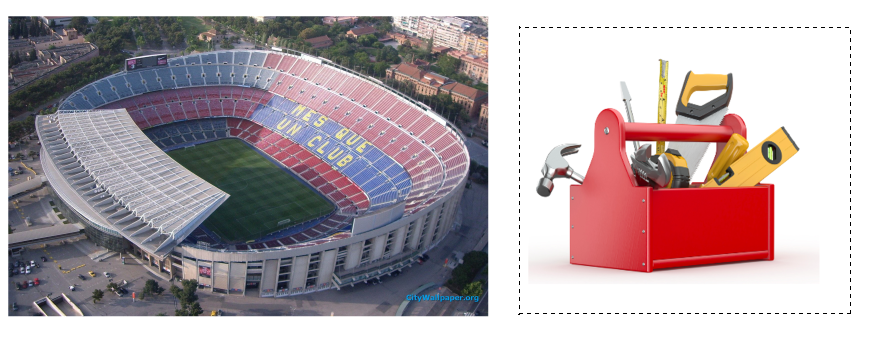
\includegraphics[scale=0.45]{img/vaa.png}
\end{center}

\begin{itemize}
	\item Nuestro 'campo de juego' no será tan increíble, exitoso y espectacular como el que aparece en la imagen. Será $\A^n_K$, o también llamado espacio afín de dimensión $n$ sobre un cuerpo $\K$ (tuplas sobre un cuerpo $\K$). Como un ejemplo vale más que x palabras con x tendiendo a 100, os pongo uno: $\A^2_{\real}$ es el plano, y las tuplas son los puntos $(x,y)$ del plano.
	\item Las herramientas serán lo que hemos dado hasta ahora, anillos noetherianos, dominios de integración, dominios de factorización única... Que empiece el juego.
\end{itemize}

\begin{defn}[Variedad algebraica]\label{def:variedad_algebraica}
	Diremos que un subconjunto $X\subset \A^n_K$ es una variedad algebraica afín si los puntos de $X$ son las soluciones de alguna colección $F$ de polinomios en $\K[x_1,...,x_n]$.

	Es decir, $X$ es una variedad algebraica afín (v.a.a.) si existe $F \subset K[x_1,...,x_n]$ tal que $X=\{ (a_1,...,a_n) \in \A_K^n: p(a_1,...,a_n)=0,  \forall p(x_1,...,x_n) \in F \} = \V(F)=\text{ 'Conjunto de soluciones de F '}$.
\end{defn}

En resumen, a grandes rasgos y para entendernos tenemos que:
\begin{itemize}
	\item Una variedad algebraica no es más que un conjunto de puntos que son solución de unas ecuaciones dadas.
	\item Dada una variedad algebraica, existe un conjunto de ecuaciones que tienen por solución los puntos pertenecientes a dicha variedad algebraica.
\end{itemize}

Vemos algunos ejemplos de variedades algebraicas afines.
\begin{example}
	\begin{itemize}
		\item $\emptyset = \V(1)$. La ecuación $1=0$ no tiene solución. $\emptyset$ siempre es una v.a.a.
		\item $\A_K^n=\V(0)$. Todos los puntos del espacio afín son solución de la ecuación $0=0$. $\A_K^n$ siempre es una v.a.a.
		\item Ahora cogemos $A^1_k$, que es la recta afín sobre un cuerpo K (por ejemplo si el cuerpo fuera $\real$, este espacio afín serían todos los puntos de $\real^1$).

		Si cojo $F=\{p(x)\}$, la variedad algebraica afín serán los puntos que son solución de la ecuación $p(x)=0$. Es decir, $\V(F)$ puede ser $\emptyset$ o un número finito de puntos, como mucho tantos como el grado de $p(x)$.
		\item Ahora vamos a coger una variedad afín y vamos a encontrar $F$. Es decir, cogemos un conjunto de puntos y buscamos qué ecuaciones son soluciones de todos a la vez.

		Por ejemplo: Sea $\K=\real$, $\{1,2,3\} =\V((x-1)(x-2)(x-3))$. Que no es lo mismo que: $\V(x-1,x-2,x-3)=\emptyset$, ya que no hay ningún valor $x$ tal que esas 3 ecuaciones sean 0 a la vez.

		De hecho la variedad algebraica anterior es más grande que lo que hemos dicho, sería: $\{1,2,3\} =\V(\gen{(x-1)(x-2)(x-3)})$. Recordemos que $\gen{(x-1)(x-2)(x-3)} = \{ p(x)(x-1)(x-2)(x-3) : p(x) \in \real[x] \}$ (todos los múltiplos de $(x-1)(x-2)(x-3)$)
	\end{itemize}
\end{example}

\obs Todo conjunto finito de puntos en $\A_K^n$ es una variedad algebraica.

\obs Sea $Y$ una colección infinita de puntos en $A^1_n$ (distinta del total), entonces $Y$ NO es una variedad algebraica afín. Ya que el conjunto de soluciones de $p(x)=0$ está acotado por el grado de $p(x)$, así que salvo que $Y=\A^n_k$, $Y$ no puede ser una v.a.a.

Así, sin mucho esfuerzo hemos descrito todas las variedades afines de la recta, que son el vacío, el total, y conjuntos finitos de puntos.

Ahora vamos a pensar en  $\A_K^2$:
\begin{example}
Sea $\A_K^2$, entonces tenemos $K[x_1,x_2]$. Vamos a buscar $F$ para:

\begin{enumerate}
\item $(a_1,a_2) \in \A^2_k$.

Probamos con $F=\{(x_1-a_1)(x_2-a_2)\}$. Que no es lo que buscamos ya que $(x_1-a_1)(x_2-a_2)=0$ tiene por solución dos rectas (las de color azul):

\begin{center}
	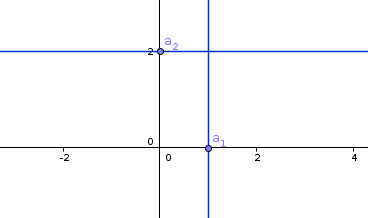
\includegraphics[scale=0.45]{img/ej1.png}
\end{center}

La solución buena es:  $F=\{(x_1-a_1),(x_2-a_2)\}$ ya que el sistema de ecuaciones $(x_1-a_1)=0$ y $(x_2-a_2)=0$ tiene como solución el punto de intersección de ambas rectas que es precisamente $(a_1,a_2)$.

\begin{center}
	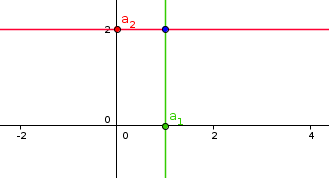
\includegraphics[scale=0.45]{img/ej2.png}
\end{center}


\item $(a_1,a_2),(b_1,b_2) \in \A^2_k$. Buscamos $F$

Se nos ocurre probar con:
\[
\left.
\begin{array}{rcl}
	(x_1-a_1)(x_2-b_2) & = & 0  \text{ \textcolor{green}{-----}}\\
	(x_2-a_2)(x_1-b_1) & = & 0 \text{ \textcolor{red}{-----}}
\end{array}
\right\}
\]

\begin{center}
	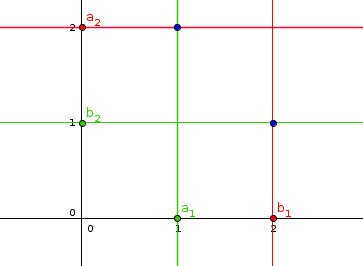
\includegraphics[scale=0.45]{img/ej3.png}
\end{center}

Que vale como solución salvo si $b_2=a_2$ o $a_1=b_1$ en cuyo caso nos saldría una recta como solución, que difiere de lo que buscamos que son dos puntos.

La solución buena es:
\[
\left.
\begin{array}{rcl}
(x_1-a_1)(x_2-b_2) & = & 0 \text{ \textcolor{green}{-----}}\\
(x_2-a_2)(x_1-b_1) & = & 0 \text{ \textcolor{red}{-----}}\\
(x_1-a_1)(x_1-b_1) & = & 0 \text{ \textcolor{black}{-----}}\\
(x_2-a_2)(x_2-b_2) & = & 0 \text{ \textcolor{purple}{-----}}
\end{array}
\right\}
\]

Que gráficamente es superponer el dibujo anterior con este:

\begin{center}
	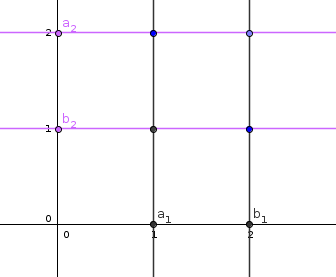
\includegraphics[scale=0.45]{img/ej4.png}
\end{center}

Por tanto $F=\{ (x_1-a_1)(x_2-b_2), (x_2-a_2)(x_1-b_1), (x_1-a_1)(x_1-b_1), (x_2-a_2)(x_2-b_2)  \}$
\end{enumerate}
\end{example}


\begin{prop}
	Sea $F \subset \K[x_1,...,x_n]$ no vacío. Entonces $\V(F)=\V(\gen{F})$.
\end{prop}

\begin{proof}
	\begin{itemize}
		\item $F \subseteq \gen{F} \implies \V(F) \supset \V(\gen{F})$. Es obvio, ya que en $\gen{F}$ hay más ecuaciones que cumplir que en $F$.
		\item Vamos a ver la otra inclusión: $\V(F) \supset \V(\gen{F})$.

		Sea $(a_1,...,a_n) \in \V(F) \implies \forall p(x_1,..,x_n) \in F$, $p(a_1,...,a_n)=0$. Y para que $(a_1,...,a_n) \in \V(\gen{F})$ tenemos que ver que $\forall q(x_1,...,x_n)\in \gen{F}$, $q(a_1,...,a_n)=0$.

		Si $q(x_1,...,x_n)\in \gen{F} \implies \exists c_1(x_1,...,x_n),...,c_s(x_1,...,x_n) \in F$ y $\exists b_1(x_1,...,x_n),...,b_s(x_1,...,x_n) \in \K[x_1,..,x_n]$ tal que $q(x_1,...,x_n)=b_1c_1+...+b_sc_s$.

		Entonces $q(a_1,...,a_n)=b_1(a_1,...,a_n)c_1(a_1,...,a_n)+...+b_s(a_1,...,a_n)c_s(a_1,...,a_n) = 0$  ya que $c_i=0$.
	\end{itemize}

	Nos falta el caso de que $\V(F)=\emptyset$. Pero el $\emptyset$ está contenido en cualquier conjunto.
\end{proof}

Pero... ¿por qué es interesante que $\V(F)=\V(\gen{F}$?

Como $\gen{F}\subset \K[x_1,...,x_n] \implies \gen{F}$ es finitamente generado, es decir, existe $p_1(x_1,...,x_n),...,p_t(x_1,...,x_n)$ tal que $\gen{F} = \gen{p-1(x_1,...,x_n),...,p_t(x_1,...,x_n)} \implies \V(F)=\V(\gen{F})=\V(p_1(x_1,...,x_n),...,p_t(x_1,...,x_n))$:

\obs Toda v.a.a. es el conjunto de solución de un nº finito de ecuaciones polinómicas.

\section{Topología de Zanski en \Akn}
Sea $\Akn$, entonces tanto $\emptyset$ como $\Akn$ son v.a.a., además $\emptyset=\V(\gen{1})$ y $\Akn=\V(0)$.


\begin{itemize}
	\item Sean $X_1$ y $X_2$ dos v.a.a. $\implies$ $X_1 \cap X_2$ es v.a.a..

	Esto es cierto ya que $X_1=\V(I_1)$ y $X_2=\V(I_2)$ para $I_1,I_2$ ideales en $\K[x_1,...,x_n] \implies$
	$$X_1 \cap X_2 = \V(I_1 \cup I_2)=\V(I_1+I_2)$$

	\textcolor{red}{$X_1$ y $X_2$ son ideales porque hemos visto que $\V(F)=\V(\gen{F})$, y $K[x_1,..,x_n]$ es noetheriano y por tanto cualquier ideal es finitamente generado}

	Conclusiones:
	\begin{enumerate}
		\item La intersección de un número finito de v.a.a. es una v.a.a.
		\item La intersección infinita de v.a.a. también es v.a.a.: Sea $\{ X_i \}_{i\in I}$ una colección de v.a.a., entonces:
		\[ \cap_{i\in I}X_i = \V(\gen{I_i, i \in I}) \]
	\end{enumerate}
	\item Sean $X_1, X_2$ dos v.a.a. $\implies X_1 \cup X_2$ es v.a.a..

	De hecho sea  $X_1=\V(I_1)$ y $X_2=\V(I_2)$,  para $I_1=\gen{f_1,...,f_s},I_2=\gen{g_1,...,g_t}$ ideales en $\K[x_1,...,x_n]$ entonces
	$$X_1 \cup X_2=\V(I_1 \cap I_2)=\V(I_1 \cdot I_2)=\gen{f_i, g_j}$$

	Conclusiones
	\begin{enumerate}
		\item La unión de un número finito de v.a.a. es una v.a.a.
		\item La unión arbitraria infinita de v.a.a. no tiene porque ser v.a.a. (Todos los enteros de $\ent$ no son v.a.a.)
	\end{enumerate}
\end{itemize}

Todo esto que hemos visto son una serie de conjeturas que son ciertas pero que aún no vamos a demostrar.

Nos quedamos con la siguiente proposición:

\begin{prop}
	Las variedades algebraicas afines satisfacen los axiomas de los cerrados de una topología. En $\Akn$ definimos la topología de Zanski, como aquella en la que los cerrados son variedades algebraicas afines.
\end{prop}

\begin{example}
	Topología de Zanski en $\A^1_K$:
	\begin{itemize}
		\item Cerrados: $\emptyset$, $\A^1_K$ y $\{ p_1,...,p_n \} \subset \A^1_K$ (cantidad finita de puntos).
		\item Abiertos: (los complementarios de los cerrados) $\A^1_K$, $\emptyset$, y el complementario de una cantidad finita de puntos.
	\end{itemize}
\end{example}

